%%%%%%%%%%%%%%%%%%%%%%%%%%%%%%%%%%%%%%%%%%%%%%%%%
%
%	MSc THESIS TEMPLATE
%	developed for my master thesis at the Universit� di Torino
%
%	by Eugenio Senes (eugenio.senes@gmail.com)
%
%	released under MIT license, so share, modify and enjoy, but quoting the author !
%
%%%%%%%%%%%%%%%%%%%%%%%%%%%%%%%%%%%%%%%%%%%%%%%%%

%% DOCUMENT CLASS (alternative to book is 'report')
% Print just right page or both sides (comment the other one)
\documentclass[12pt,a4paper,openright,oneside]{book}  %%One sided

%% SET MARGINS OF THE PAGES
\usepackage{geometry}
\geometry{a4paper,portrait, left=40mm, right=30mm, top=35mm, bottom=30mm}

%% HEADERS AND FOOTERS
\usepackage{fancyhdr}
\pagestyle{fancy}
\fancyhf{} %clears default header and footer
\rhead{} %right head
\lhead{ \leftmark} %left head
\rfoot{\thepage}
%%consider using also chead, cfoot, lfoot
%coherce the plain stile to this (e.g. the first page of every chapter)
\fancypagestyle{plain}{
	\fancyhf{}
	\rfoot{\thepage}
	\renewcommand{\headrulewidth}{0pt}
	\renewcommand{\footrulewidth}{0pt}
}
%% CLEAR PAGE WITHOUT NUMBER AT THE BEGINNING OF CHAPTERS
\let\origdoublepage\cleardoublepage
\newcommand{\clearemptydoublepage}{%
  \clearpage
  {\pagestyle{empty}\origdoublepage}%
}
%% ALLOW PAGE ROTATION
\usepackage{lscape}

%% HYPERTEXT SETUP
\usepackage{hyperref}
\hypersetup{
    colorlinks,
    citecolor=black,
    filecolor=black,
    linkcolor=black,
    urlcolor=black
}
%% PDF SETTINGS
\hypersetup
{
    pdfauthor={AuthorName},
    pdftitle={shortTitle},
    pdfsubject={subject},
    pdfkeywords={keyword1, keyword2}
}
%% FONTS AND SYMBOLS
\usepackage[utf8]{inputenc}	%%input font setting
\usepackage[T1]{fontenc} 		%%font for automatic recognition of letters with the accent
\usepackage{amsfonts}		%%fonts for the mathematical rendering of formulas
\usepackage{amssymb}
\usepackage{amsmath}
\usepackage{ mathrsfs }
%% CHAPTERS STRUCTURE
\usepackage[italian,english]{babel} %%Set English as main language of the document
%% FIGURES
\usepackage{graphicx}
\usepackage{subfigure}	%%Allow side by side figure
%%CAPTIONS
\usepackage{caption}
%% BIBLIOGRAPHY
\usepackage[babel]{csquotes}

%% TABLES
\usepackage{multirow}

%% HYPENATON
\hyphenation{de-ve-lop-ment ac-ce-le-ra-ting de-ve-lo-ping bend-ing wa-ve-gui-de}

%%%%%%%%%%%%%%%%%%%%%%%%%%%%%%%%%%%%%%%%%%%%%%%%%
%%%% BEGIN DOCUMENT
\begin{document}

%%%% HEAD  OF THE DOCUMENT
\frontmatter
%%FRONT PAGE
\begin{titlepage}
%upper part
\begin{center}
{{\Large{\textsc{Universit\`a degli studi di Torino \\}}}} \vspace{5mm} {\small{\bf SCUOLA DI SCIENZE DELLA NATURA\\ \vspace{3mm}
Corso di Laurea Magistrale in Fisica}}
\vspace{5mm}
\end{center}
%logo
\begin{center}

\includegraphics[scale=.3]{head/logo.png}
\end{center}
%title
\begin{center}
\vspace{5mm}
{\large{\bf Tesi di Laurea Magistrale\\}}
\vspace{5mm}
{\LARGE{\bf TEST OF THE BEAM EFFECT ON VACUUM ARC OCCURRENCE IN HIGH-GRADIENT ACCELERATING STRUCTURE FOR THE CLIC PROJECT\\}}
%\vspace{5mm}
%{\LARGE{\bf SECOND ROW TITLE}}
\end{center}
%reatori e candidato
\vspace{11mm}
\par
\noindent
\begin{minipage}[t]{0.47\textwidth}
{\large{\bf Relatore:\\
Prof. Martino Gagliardi}}\\
\vspace{4mm}
\\
{\large{\bf Co-relatore:\\
Dr. Frank Tecker (CERN)}}
\vspace{8mm}
{\large{\bf \\ Controrelatore:\\
Prof. Ferruccio Balestra}}
\end{minipage}
\hfill
\begin{minipage}[t]{0.47\textwidth}\raggedleft
\vspace{16mm}
{\large{\bf Candidato:\\
Eugenio Senes}}
\end{minipage}
\vspace{9mm}
\begin{center}
{\large{\bf 
Anno Accademico 2015/2016}}
\end{center}

\end{titlepage}
\clearemptydoublepage
%%DEDICATION (the initial quote)
\thispagestyle{empty}
\begin{flushright}

\vspace*{60mm}

The amazing quote\\
that I chose as inspiration\\
for this work\\
\vspace{4mm}
Author, \textit{Title}\\




\end{flushright}
\clearemptydoublepage
%%ABSTRACT
\chapter*{Abstract}

\begin{center}
\textit{(Leave this for the moment ....)}
\vspace{4cm}
\end{center}



A new generation of colliders capable of reaching TeV energies is under development nowadays, and to succede in this task is necessary to show that the technology for such machine is available. The CLIC project is one of the most advanced design among the possible lepton colliders, and is formed by two normal conducting LINACs. To reach such high energies are necessary accelerating structures carrying gradient beyond 100MV/m and one of the biggest limitations is developing accelerating structures that present a sufficient low occurrence of vacuum arcs. This is pursued both with the design and the \textit{conditioning}, which is the process of increasing the resilience to vacuum arcs of a structure using repetitive RF pulsing sessions. 

The focus of this work is on the breakdown rate testing of the TD26 type cavity with and without beam presence inside. At CERN this test has been carried out on the cavity installed in the \textit{dogleg} line in the CLIC-test-facility 3 (CTF3), and connected on the RF side to the X-band test stand 1 (Xbox1).

Other peculiar properties of the operation have been studied also, such has beam-induced RF generation into the cavity after the breakdowns, breakdown migration, ....
\chapter*{Italian abstract}

Una nuova generazione di acceleratori di leptoni capaci di raggiungere energie del centro di massa dell'ordine del TeV é al momento in corso di sviluppo, e  per avere successo in questo compito, é necessario mostrare che la tecnologia per costruire macchine di questo tipo é disponibile.

Il Compact Linear Collider (CLIC) é uno dei possibili progetti tra i futuri acceleratori di leptoni. CLIC consiste in due linac normalmente conduttivi. Strutture di accelerazione con gradienti dell'ordine dei 100 MV/m sono necessarie per raggiungere le alte energie richieste, mantenendo una lunghezza della macchina ragionevole. Uno dei parametri pi\`u stringenti per queste strutture di accelerazione é una occorrenza relativamente bassa di archi voltaici nel vuoto.

Prototipi di strutture di accelerazione per CLIC sono gi\`a stati testati in passato, ma solo in assenza di fascio. Per provare la fattibilit\`a della tecnologia di accelerazione ad alto gradiente, in modo da costruire un acceleratore funzionale, é necessario comprendere l'effetto della presenza del fascio sull'occorrenza di archi voltaici nel vuoto. Test di questo tipo non sono mai stati effettuati fino ad ora.

L'obiettivo principale di questo lavoro é fornire una prima misura del rate di occorrenza degli archi voltaici in una cavit\`a acceleratrice in presenza di fascio. Verranno descritti il setup, le procedure sperimentali e i risultati dei test eseguiti su un prototipo di cavit\`a acceleratrice per il fascio principale di CLIC.

I test sono stati eseguiti al CERN nella CLIC Test Facility 3 (CTF3), che ospita un setup di test per radiofrequenza ad alta potenza operante a 12 GHz (detto XBOX, X-band Test Stand). L'XBOX fornisce la radiofrequenza alla cavit\`a sotto test, mentre il fascio proviene dal linac a elettroni della CTF3, configurato per produrre un fascio simile al fascio principale di CLIC. Verr\`a presenta una comparazione tra i risultati ottenuti senza fascio e con differenti configurazioni di fascio, in un primo tentativo di comprendere l'effetto del fascio sul rate di archi voltaici. Inoltre verranno proposti sviluppi futuri per migliorare il setup sperimentale e le operazioni di test, basati sull'esperienza acquisita nei test oggetto di questo lavoro. Questo sar\`a utile, nel caso l'esperimento venisse ripetuto, per completare ed estendere i risultati di questo lavoro.
\clearemptydoublepage
%%INDEXES
%summary
\tableofcontents
\clearemptydoublepage
%%%% BODY OF THE DOCUMENT
\mainmatter
%%INTRODUCTION
\chapter{Introduction}
Particle accelerators occupy a key role both in fundamental research and in all the applications and industrial processes that uses technology and processes developed initially for the elementary research.

In the fundamental research, accelerators are central to inquire the world at the elementary particle scale. But also the contribution given to the other sciences does not have to be forgotten.
In fact a number of examples could be named among the spin-offs of accelerator science, the most notable nowadays is the enormous progress of nanosciences in the last decade. That was made possible by the availability of high-brilliance synchrotron light sources, that were achievable thanks to the experience developed in the production of high quality electron beams. In the same way inquiring a much smaller scale requires machines involving higher energies.
 Hence in this perspective keeping developing the accelerators for the physical research is a fundamental requirement to assure that the cutting-edge technology of today turns into the "labware" of tomorrow for all the other sciences and industry.

Going back to the particle scale, at the moment the most successful model to explain the behaviour of the elementary particles is the \textit{Standard Model}, but it is not conclusive and not able to answer all the questions still open in particle physics. A milestone in favour of the Standard Model was the observation of the Higgs Boson in 2012 \cite{CMS:higgs,ATLAS:higgs}, which was made possible by the construction of the \textit{Large Hadron Collider} at CERN\cite{LHC:design}. However the full understanding of the physics at the particle scale still needs to be achieved. Partially this will be realised with the continued data taking of the LHC, but also the International Committee for Future Accelerators (ICFA) considers that the results of LHC need to be complemented by the results of a lepton collider in the TeV-range\cite{ICFA:linStat}.

The reason for this is that according to the standard model the hadrons are particles composed of quarks, that are continously interacting exchanging gluons. This particularity causes the collisions at high energy to be between partons. In addition, there is no  way \textit{a priori} to know the energy of the partons involved, so it is impossible to know which will be the energy of the collision. For example it is improbable for a parton in the 14 TeV centre-of-mass energy LHC to have much more than 1-2 TeV of energy at the interaction point\cite{LHC:partonDistrib}. On the other hand, the leptons are pointlike particles, so the interaction is directly involving the two bullets themselves at a given energy, and the number of possible processes that can take place is definitely smaller. 

This key difference in the behaviour of leptons and hadrons makes hadron colliders \textit{machines for discovery}, because it involves all the possible processes that can take place in a wide range of energies, and the lepton machines \textit{machines for precision}, because the reduced number of possible processes makes the observation of the events of interest much easier.

\section{Generalities on colliders}

According to the beam setup two kinds of accelerators can be distinguished: 
\begin{enumerate}
\item Fixed target: where a beam is shot against a non-moving target. The energy in the centre-of-mass is $E_{CM} \propto \sqrt{E_{BEAM}}$
\item Colliders: where two beams are accelerated in opposite directions and then made collide with each other. In the case of equal beam energy, in the centre-of-mass $E_{CM} = 2 E_{BEAM}$
\end{enumerate}
Therefore it is easy to see that the collider topology is preferable to reach a high centre-of-mass energy.

In the collisions, the rate of observation of a particular interaction process A is given by
\begin{equation}
\frac{dN(A)}{dt} = \mathscr{L} \, \sigma(A)
\end{equation}
where $\sigma$ is the process cross-section, which depends by the physics of the process A itself, and $\mathscr{L}$ is the luminosity, which depends entirely on the accelerator.
Therefore the figure of merit when it comes to talk about accelerators is the luminosity, which is given by
\begin{equation}
\mathscr{L} = H_d \frac{N^2}{\sigma_x \sigma_y} n_b f_r
\end{equation}
where $N$ is the number of particles per bunch, $\sigma_x$ and $\sigma_y$ are the beam dimensions in the horizontal and vertical plane, $n_b$ is the number of bunches, $f_r$ is the collision frequency of the bunches and $H_d$ is a correction factor that takes in account the non-ideality of the collision, such as crossing angle, collision offset, hour glass effect, non gaussian beam profile and so on.

It is necessary to reach the highest luminosity possible since the events that are going to be studied are rare. This is realised differently according to the design of the accelerator in use:
\begin{itemize}
\item linear accelerators (linacs): have a low repetition frequency, typically lower than hundreds of Hz, and the beam is passing just once to be accelerated through the machine.
\item circular accelerators (typically synchrotrons): have a higher repetition frequency, up to tenth of kHz, and are keeping the particle beam in orbit for many turns, so can accelerate it over a long period of time.
\end{itemize}
After this distinction one could be led to think that the circular machine is the best choice in any case in order to reach high luminosity, but raising the energy of the beam becomes problematic: in fact the power loss in circular collider due to the emission of synchrotron radiation scales according to the following expression
\begin{equation}
P \propto \frac{1}{\rho^2} \frac{E^4}{m_0^4}
\end{equation}
where $\rho$ is the bending radius of the machine, $E$ is the particle energy and $m_0$ is its rest mass. The power loss becomes very important for electrons and positrons, as can be noted in Table \ref{table_CLIC_ILC_FCC}, the energy loss per turn is a relevant fraction of the beam energy, e.g. for the LEP collider, at the highest  energy per beam of 104.5 GeV, more than 3 GeV were lost per turn. To raise the beam energy and reduce the energy loss, the radius of circular machines escalates quickly. Simply scaling LEP, it is possible to show that in order to reach the centre-of-mass energy of 3 TeV, the circumference should be increased to thousands of kilometers \cite{nature:CLIC}.
To solve the issue, the development of new lepton colliders is focusing on two different solutions:
\begin{enumerate}
\item Use muons instead of electrons: this innovative approach reduces the power lost because of the higher mass of the muon compared to the electron, but one has to deal with the short lifetime of muons, which is roughly $2 \, \mu s$ in the rest frame.
\item Limit the losses caused by synchrotron radiation, either by increasing the bending radius or abandoning the circular topology for the linear one.
\end{enumerate}
It has to be noted that the muon technology is rather new and still needs to be fully developed, while the linear accelerator technology profits of the progress achieved in the last half century mainly in CERN, SLAC and KEK.

In this perspective a number of projects are under study at the moment, of which the most ambitious are FCC-ee, \textit{Future Circular Collider}, ILC, \textit{International Linear Collider}, and CLIC, \textit{Compact Linear Collider}. The first one consists of a circular collider which is supposed to be placed in a 80-100 km long tunnel before the installation of the FCC-hh, the others are linacs even if based on completely different technologies and solutions.  A comparison of the features of these projects in the final stage is presented in table \ref{table_CLIC_ILC_FCC}, together with LEP as an example of a circular lepton collider.

\begin{table}
  \centering
    \begin{tabular}{ l c c | c c c }
    \hline
    \hline
    \textbf{Parameter}								& \textbf{LEP2}	&	\textbf{FCC-ee}	&  \multicolumn{2}{c}{\textbf{CLIC}}	&	\textbf{ILC}	\\
    \hline
    $\sqrt{s}$ [GeV]								& 209	& 350  			&  	500	&  3000	& 500	\\
    $\mathscr{L}_{peak}$  $[10^{34} \, \text{cm}^{-2} \, \text{s}^{-1}]$	&0.012	& 1.3				&  	2.3	& 	5.9	&1.8		\\
    Total length [km]								&26.7	& 100			& 13		&  48.4	& 31		\\
    $E_{acc}^{loaded}$ [MV/m]						& 5 - 9	& 10 - 20			& 80		& 100 	& 31.5	\\
    Bunch population $[10^9]$						& 105	& 170  			&  6.8	& 	3.72	& 500	\\
    Bunch spacing [ns]							& 		& 4000	  		&  	0.5	& 	0.5	& 554	\\
    Collision rate [Hz]								&  		&$\approx$ 3000	&  	50	& 	50	& 5		\\
    $\epsilon^*_x \, / \, \epsilon^*_y $ [$\mu$m]/[nm]		& 		&  	0.68/0.68	        		&  2.4/25	& 0.66/20	& 10/35	\\  
    $\sigma^*_x\, / \, \sigma^*_y$ [nm]				& 		&  	3600/70		&  202/2.3	& 40/1	&474/5.9	\\    
    Energy loss [GeV turn$^{-1}$]					&  3.34	& 	7.55			& - 		& -		& -		\\
    AC Power [MW]								&  120	& $\approx$ 300		& 271	& 582	& 163	\\
    \hline
    \hline
    \label{CLIC_param_table}
    \end{tabular}
  \caption{Comparison of two circular machines, LEP\cite{Aull:2156972,LEP:RF} and FCC-ee\cite{FCC-ee:leptonCollParam,Zimmermann:2057706} and the two projects for linear machines, the first and last stage of the CLIC implementation \cite{CLIC:cdr} and the ILC\cite{ILC:tdr} }\label{table_CLIC_ILC_FCC}
\end{table}



Furthermore a recent interest arose in more compact technologies, e.g. plasma acceleration techniques, but the reliability of such designs still needs to be proven in the perspective of creating a fully functional machine that goes beyond the demonstration of the working physical principle.



\section{The CLIC project and the CTF3 facility}

The \textit{Compact Linear Collider} is the project for a linear electron-positron collider capable of reaching a centre-of-mass collision energy of 3 TeV and a luminosity of $2\text{x}10^{34} \, \text{cm}^{-2} \, \text{s}^{-1}$ in the final stage.

\subsection{Physics and staging}

The machine is designed to be built in 3 stages, with a final energy of 3 TeV. 

Since the Conceptual Design Report (CDR)\cite{CLIC:cdr} was released just before the discovery of the Higgs boson, the centre of mass energy stages have been reshaped in order to be able to access interesting measurements. For a given centre-of-mass energy stage, the energy can be modified by a third with limited loss of performance\cite{CLIC:cdrVol3}, allowing an eventual retuning of the energy of the stages following the results of the LHC physics campaign.

The energy staging has been chosen with the idea to access the Higgs and top physics from the first stage \cite{CLIC:staging2016,Bozovic-Jelisavcic:2160172}.

In the first stage at 380 GeV the measurements on the Higgs physics can be conducted through Higgsstrahlung and WW-fusion processes, thereby providing accurate model-independent measurements of Higgs couplings to bosons and fermions\cite{Roloff:2210491}; the top physics measurements will be focused on the $t\bar{t}$ pair production threshold in the vicinity of $\sqrt{s} = $ 350 GeV.

The second stage is proposed at 1.5 TeV and allows to access new physics phenomena and additional properties of the Higgs boson and the top quark, such as Higgs self-coupling and rare Higgs branching ratios.

The third stage is proposed at 3 TeV and will give direct access to pair-produced particles with mass up to 1.5 TeV or single particles with mass up to 3 TeV. This stage is particularly interesting as test for the Beyond Standard Model theories, since such high energy in a lepton machine makes the observation of new particles much easier than in the LHC.

A further adaptation of these steps is possible after the publication of the results of the run 2 of the LHC. In any case the advantage of a linear machine in this sense is that the final energy can be reshaped modifying the total length of the machine. Figure \ref{CLIC_map} showS the footprint of a possible CLIC built in the Geneva area, in order to give an idea about the order of magnitude of that kind of facility compared to LHC.

\begin{figure}[h]
\centering

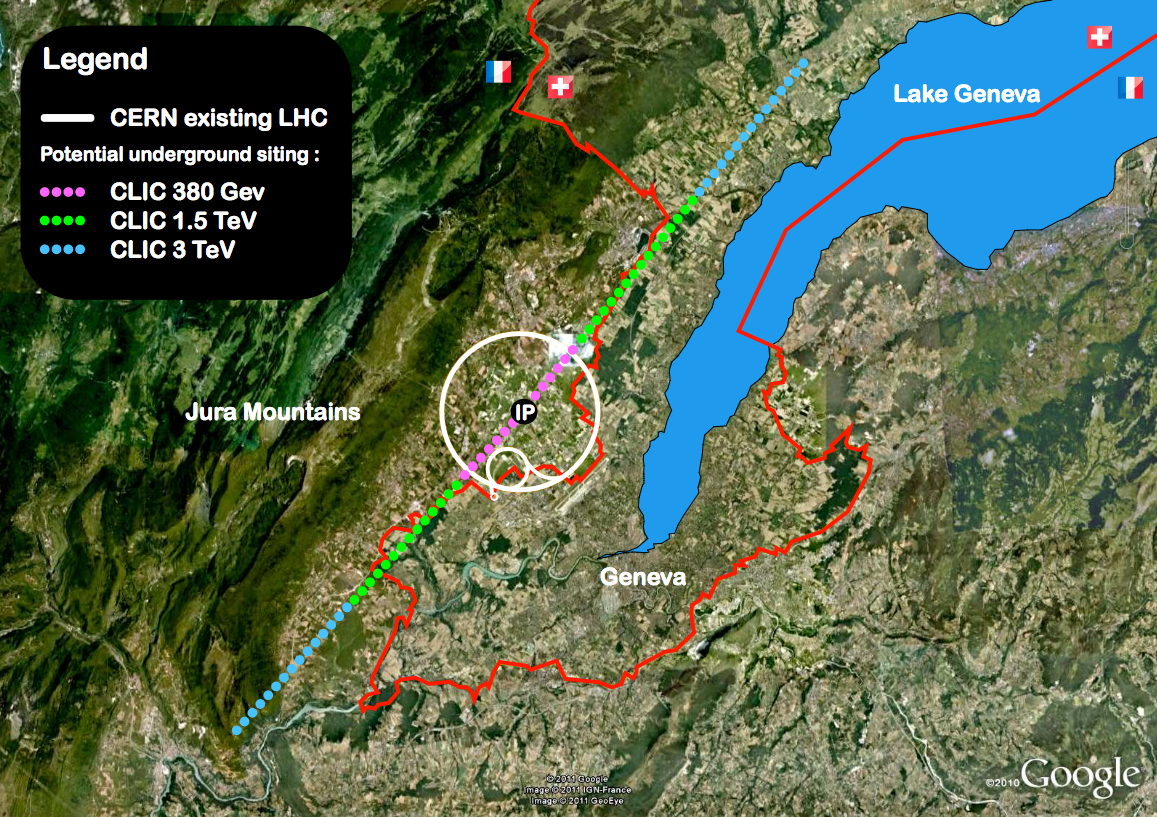
\includegraphics[scale=0.3]{pictures/CLIC_map}
\caption{Map of the CLIC facility, if implemented in the Geneva area.}
\label{CLIC_map}

\end{figure}


\subsection{Main parameters and main issues}

The realisation of such machine implies many technological challenges in order to keep the power consumption and the dimension limited while matching the design goal parameters. These challenges have been faced developing the novel \textit{two-beam acceleration scheme}, in which the idea is to use a high-current and low-energy beam, the \textit{Drive Beam}, in order to generate the RF power to accelerate a low-current and high-energy beam used for the experiments, named \textit{Main Beam}. \\
The Drive Beam is produced using a dedicated linac, and then the current is multiplied using a delay loop and two recombination rings, reaching a combination factor of $2\text{x}3\text{x}4=24$. This topology generates the beam with a final frequency of the bunches of 12 GHz. It is essential to reach the highest possible efficiency in the Drive Beam production, in order to shrink the power consumption to the smallest possible. To reach this goal the acceleration in the linac is performed using the accelerating cavities in fully-loaded mode \cite{Corsini:791372}.

While the biggest challenge for the Drive Beam is reaching the necessary stable high current, for the Main Beam the hardest challenge is generating a beam with the smallest dimension possible, in order to increase the luminosity of the machine as much as possible.\\
The Main Beam is produced in a separate facility, where a DC-photo gun system provides the initial polarised electron beam. The positron beam is generated by another electron beam hitting a target. Once both beams have been produced, they are sent to the next accelerating stages, which are composed of linacs to raise the beam's energy and of damping rings to reduce the emittances. 

The detailed description of the Main Beam production and the Drive Beam recombination process can be found in \cite{CLIC:cdr}. The working principle has been demonstrated in the CTF3 \cite{CTF:drive_beam}. 

Both beams are sent to the common tunnel where the Two-beam modules are installed. The Two-beam module is composed of two principal sections, which are the PETS, \textit{Power Extraction and Transfer Structures}, and the accelerating structures for the Main Beam, as shown in figure \ref{TBM}. The Main Drive passes through the PETS and gets decelerated. As product of the deceleration a pulse of RF power is produced, which is transferred by a waveguide network and used to accelerate the Main Beam.\\ In this way it is possible to reach an efficient acceleration of the Main Beam up to the desired energy for the experiments.

\begin{figure}[h]
\centering

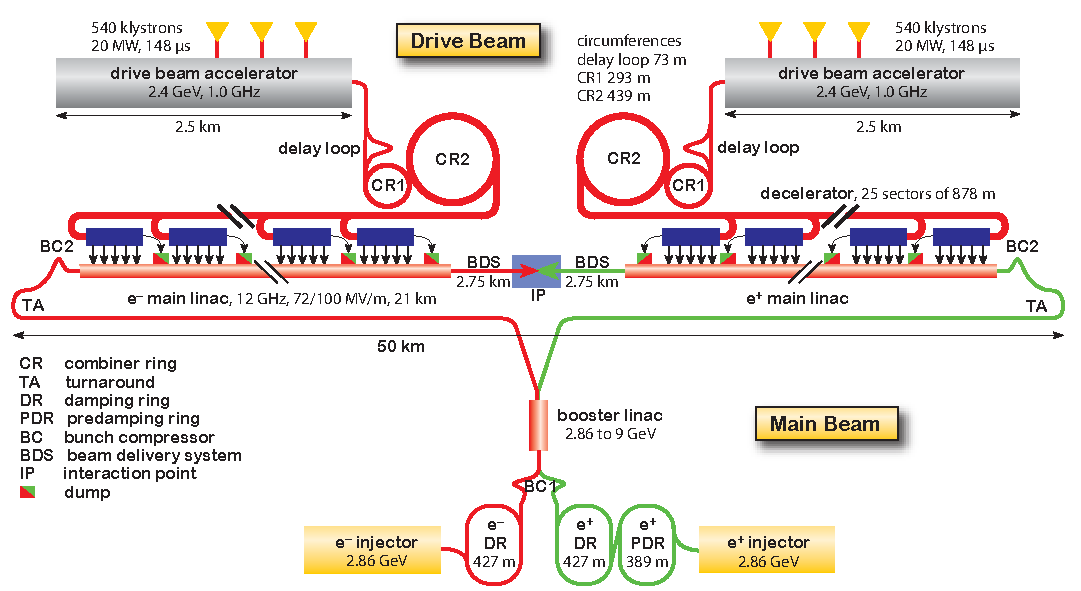
\includegraphics[scale=0.39]{pictures/CLIC_layout_3Tev}
\caption{Layout of the final stage of CLIC.}
\label{CLIC_layout}

\end{figure}

\begin{figure}

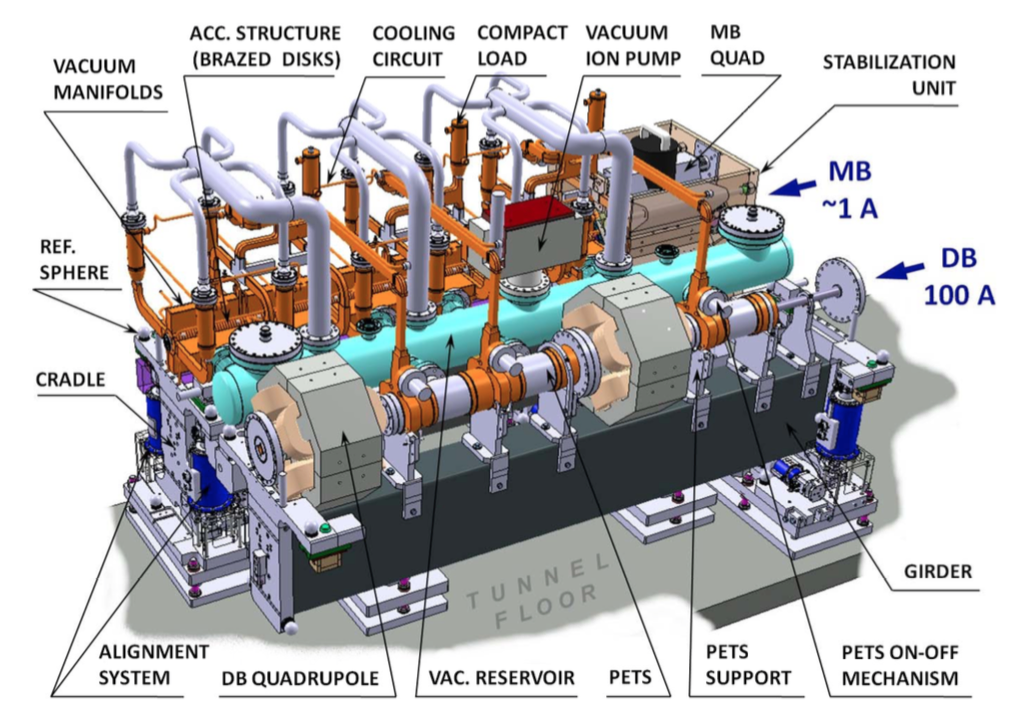
\includegraphics[scale=0.39]{pictures/TBM}
\caption{Design of a Two-beam module. }
\label{TBM}

\end{figure}







There are many issues that can affect the performance of a machine like CLIC, and need to be analysed carefully since no similar machine has been built so far. 

The main issues are:

\begin{enumerate}
\item 100 MV/m accelerating gradient: this requirement comes from the final energy of 3 TeV and the requirement of a maximum length of 50 km.
\item Breakdown rate $< 3\text{x}10^{-7}$ breakdowns per pulse per meter: this limitation comes from the limit on design luminosity loss in case of breakdown. This is the aim of this work and will be stressed in detail later.
\item Transverse wakefields limitation: wakefields have to be considered because of the short bunch spacing in the bunch train. If not limited, they are a serious issue to the luminosity.
\item Powering the accelerating structures: the klystrons on the market are not able to produce a high-power RF pulse 150-200 ns long with a high efficiency. In order to achieve a high efficiency, it is possible to use klystrons equipped with RF pulse compression systems. This option is an alternative for the first energy stage of CLIC. For higher energies, the Drive Beam option is more cost efficient.
\item Generate the drive beam with the highest efficiency in order to contain the power consumption. Also the efficiency of the power transfer between the beams is a key issue in order to reach the energy goal.
\item Extremely small beam emittance and size: in order to match the luminosity goal with the typical low repetition rate of a linac it is necessary to squeeze the beam as much as possible, reaching the goal of 40 and 1~nm at the interaction point in the horizontal and vertical plane. This parameter includes the realisation of a nanometric alignment and vibration stabilisation system.
\end{enumerate}



Therefore the parameters in table \ref{table_CLIC_params} have been selected in order to match the design parameters reported in table \ref{table_CLIC_ILC_FCC} for the top design energy.


\begin{table}[h]
  \centering
    \begin{tabular}{ l c  }
    \hline
    \hline
    \textbf{Description}						& \textbf{CLIC 3 TeV}	\\
    \hline
    Peak luminosity [cm$^{-2}$ s$^{-1}$]			& $2.0\text{x}10^{34}$	\\
    Total site length [km]						& 48.4				\\
    Loaded accelerating gradient [MV/m]			& 100	\\
    Main LINAC RF frequency	[GHz]			& 12	\\
    Number of particles per bunch				& $3.7\text{x}10^{9}$ \\
    Bunch separation [ns]						& $0.5$ \\
    Bunches per train							& $312$ \\
    Beam pulse duration [ns]					& $156$ \\
    $\epsilon^*_x \, / \, \epsilon^*_y$ [$\mu$m]/[nm]	& $0.66/20$ \\  
    $\sigma^*_x\, / \, \sigma^*_y$ [nm]			& $40/1$	\\
    
    \hline
    \hline
    \end{tabular}
  \caption{CLIC main parameters in the final stage}
\label{table_CLIC_params}
\end{table}







\subsection[CTF3]{The CLIC Test Facility 3}

To be able to affirm that the CLIC scheme is a feasible and a reliable technology to build a functional collider, a number of tests have to be conducted since no accelerators using the Two-beam acceleration concept have been built. The CLIC Test Facility 3 has been built and operated at CERN in order to demonstrate experimentally:

\begin{itemize}
\item The feasibility of the Drive Beam generation with a frequency of 12 GHz, performing the beam recobination using a delay loop and a combiner ring for a total multiplication factor of $2\times4 =8$.
\item The RF power production using the PETS and investigate possible issues of the Two-beam scheme.
\end{itemize}
In addition, a branch of the linac was used to perform high-gradient tests with the beam presence inside the accelerating cavity, which is the topic of the following work. A more detailed description will follow in chapter 4.

\clearemptydoublepage
%% CHAPTERS
% add any further chapter file here
\chapter[Accelerating structures]{Accelerating structures}

The accelerating structures are one of the key parts of a particle accelerator. Even though in the first accelerators the particle acceleration was achieved simply with fixed fields, this technique showed its limitations quite soon due to the impossibility to create arbitrary high DC voltages without being subjected to electrostatic discharges. The present conventional technology for particle acceleration is based on RF cavities, so it is natural try to push the state-of-the-art technology the furthest possible in order to reach the highest acceleration possible in the shortest length. In the case of the CLIC project a key issue is to be able to produce cavities with an accelerating gradient of 100 MV/m, which is the cutting-edge value at the moment when keeping the breakdown rate limited.

In this chapter some topics about the theory of accelerating cavities will be presented. The aim is to give to the reader a theoretical introduction to be able to understand the description of the cavity under test.

\section[Travelling wave accelerating structures]{Travelling wave accelerating structures}

In this section some useful concepts and result of the electromagnetic theory will be recalled. Because of conciseness, the examples and the geometries presented will refer to travelling wave accelerating structures, since it is the only type of structure used in this work. The curious reader can find details on the untreated topics in \cite{Weiss:261732,Wangler:RF_LINAC,Humphries:107756} and in plenty of specialised books.

\subsection[Reminder of Electromagnetism]{Reminder of Electromagnetism}

\subsubsection{Maxwell's equations}

It's well known since the basic courses of physics that the propagation of the electromagnetic fields follow the Maxwell's equations, that in a medium are
\begin{equation}
\begin{array}{l l l l}
\nabla . \vec{D} = \rho_{free}\\
\nabla . \vec{B} = 0\\
\nabla \times \vec{E} = - \frac{\partial \vec{B}}{\partial t}\\
\nabla \times \vec{H} = \vec{J}_{cond} + \frac{\partial \vec{D}}{\partial t}
\end{array}
\end{equation}
where $\vec{E}$ and $\vec{B}$ are the electric and magnetic field in the vacuum, $\vec{D} = \epsilon \vec{E}$, $\vec{B} = \mu \vec{H}$ and $\vec{E} = \sigma \vec{J}$. The propagation in vacuum is described by the same equations and can be easily derived with an appropriate choice of the constants.

\subsubsection[Waveguides and resonant cavities]{Waveguides and resonant cavities}

In some particular cases the confined propagation of electromagnetic waves is possible, and is commonly realised using a metal waveguide to direct all the energy in a single direction. In this section some useful results on the propagation in a waveguide will be stressed, the full derivation can be found in literature \cite{Botta:EM, Jackson:ClassEM,Weiss:261732}. 

The request of propagation in the direction of the axis of the waveguide can be traduced to the condition $\vec{E} \times \vec{n} = 0$, that means asking that no power is dissipated in the walls of the cavity by Joule effect since the electric field is normal to the surface anywhere and anytime.

Many solutions can be found to the problem, integrating the Maxwell's equations with the given boundary condition, but without entering in the calculations, the interesting solutions belong to two classes:
\begin{itemize}
\item \textbf{TM modes:} Transverse Magnetic modes, where the axial component of the magnetic field is null
\item \textbf{TE modes:} Transverse Electric modes, where the axial component of the electric field is null
\end{itemize}
Every mode has a particular cutoff frequency, and will propagate only in case that the condition $\omega > \omega_c$ is met (where $\omega_c = 2\pi f_c$ and $f_c$ is the cutoff frequency of the mode). The cutoff frequency of each mode depends mainly on the geometry of the guide utilised, and waves with a frequency lower than the cutoff frequency will be exponentially damped.

For particle acceleration purposes, the fundamental feature of a waveguide is that the \textit{phase velocity} is $v_p = \frac{\omega}{k} > c$, so it is not suitable for particle synchronous acceleration. The dispersion relation for a uniform waveguide can be expressed as 
\begin{equation}
\omega^2 = \omega^2_c + (k_0 \, c)^2
\end{equation}
where $\omega_c = K \, c$ and $K$ is the cutoff wavenumber.

The \textit{group velocity} instead is $v_g = \frac{\partial w}{\partial k} < c$ as expected for the physical quantity representing the speed of propagation of the EM wave according to Relativity. 
In any case, waveguides are a key building block of particle accelerators to deliver the RF power form the production equipment to the accelerating cavities.

A particular case is represented by \textit{Resonant Cavities}, which are in the simplest case closed waveguides at the terminations (e.g. a cylindrical cavity, or \textit{pillbox cavity}, is composed of a circular waveguide closed by two planes at the extremities). In resonant cavities the EM field can resonate according to the particular eigenfrequencies of the system, which are mainly dictated by the geometry. This process allows propagation of just a set of frequencies, just like in the WGs, but when a cavity is operating at one of the eigenfrequency starts to accumulate energy because of the resonance. This mechanism is utilised in accelerating structures.


\subsection[Periodic accelerating structures]{Periodic accelerating structures}

As mentioned above the waveguides themselves are not useful to accelerate particles because of the excessive phase velocity. However it's possible to reduce it loading the structure with additional metallic walls placed orthogonally to the axis of the cavity.  Such structures are named \textit{Disk (or Iris) Loaded Accelerating Structures}. A schematic example is presented in figure \ref{ACS_scheme}

\begin{figure}[h]
\centering

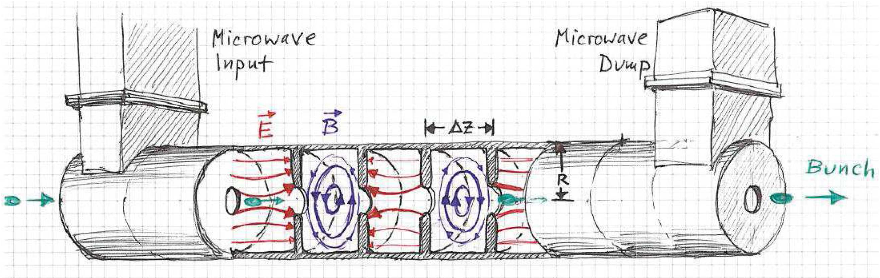
\includegraphics[scale=0.45]{pictures/scheme_ACS}
\caption{Scheme of a travelling wave, disk loaded accelerating structure. The drawings illustrates the input and output couplers, the disks loading the cavity and the beam passing through the irises. From \cite{streun}}
\label{ACS_scheme}

\end{figure}

The accelerating structure is composed of \textit{cells}, which are connected by the \textit{iris} to the adjacent cells. At the beginning and the end of the structure two special cells form the input and output coupler for the RF. The role of the irises is creating a free path for the passage of the beam and allowing the propagation of the EM field from the input coupler to the output one. In the case of room temperature cavities the material normally used is Copper, while for superconducting cavities the material can vary and also metallic cavities coated internally with a superconductive layer are a possibility.

From the field perspective, the fact that the accelerating structure is loaded with the disks changes the way that the EM waves propagate in the structure. The full mathematical description, is found in \cite{ Jackson:ClassEM,Weiss:261732}, here simply a general idea of the process and of the relevant results is given.

The geometry of the accelerating structure can be seen as a cylindrical cavity loaded regularly with the disks. If as first approximation we consider an infinite structure, it is possible to use the \textit{Floquet's Theorem}, that can be summarised as follows: \textit{"In a given mode of an infinite periodic structure, the fields at two different cross sections that are separated by one period differ only by a constant factor, which in general is a complex number"}. This has two main implications: there are some regions of the spectrum of $\omega$ that don't allow the waves to propagate, called \textit{stopbands}, and others, called \textit{passbands}, where the propagation is allowed with a \textit{phase shift} $\Delta \phi = k_0 d$, where d is the length of the cell. The phase advance per cell is a particular parameter of every structure, and is defined in the design phase.

The waves that are allowed to propagate in such conditions are called \textit{Space Harmonics}, and can be seen as an infinite number of waves propagating at the same frequency but with different wavenumbers. The dispersion relation becomes
\begin{equation}
\omega ^2 = \omega^2_c + c^2 \left( k_0 + \frac{2\pi n}{d} \right)^2
\end{equation}
where the principal wave of the mode has $n=0$ and the others have $n$ according to the direction of propagation.

The phase velocity of the n-th harmonic becomes
\begin{equation}
\beta_n = \frac{\omega}{k_n c} = \frac{\beta_0}{1+n\beta_0 \lambda/d}
\end{equation}
which allows to reach an arbitrary low phase velocity, as requested for the particle acceleration.

The comparison of the phase velocity of a waveguide and accelerating structure is presented in figure \ref{vp_fig}.



\begin{figure}[h]
\centering

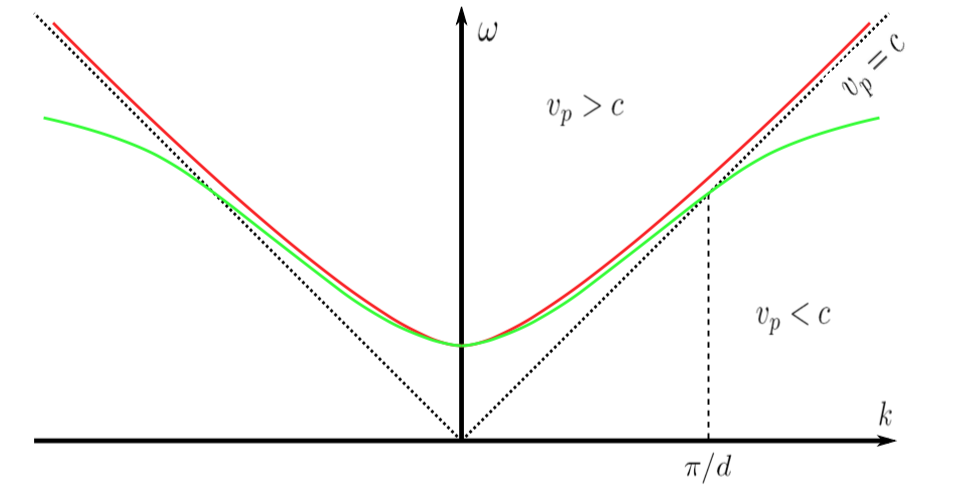
\includegraphics[scale=0.4]{pictures/vp}
\caption{Brillouin diagram of a uniform waveguide (red) compared to a disk-loaded accelerating structure (green) \cite{Kovermann:1330346}}
\label{vp_fig}

\end{figure}




\subsection[Synchronous particle acceleration]{Synchronous particle acceleration}

A particle injected in an electromagnetic field in some conditions can gain energy at expense of the field, getting accelerated. This is possible if the particle is injected at the right moment and the field and the particle have the same speed. In this manner the particle can travel with the field with an energy gain given by
\begin{equation}
\Delta W = q V_o cos \phi
\end{equation}
where $q$ is the charge of the particle, $V_0$ is the accelerating field and $\phi$ is the relative phase between particle and RF field.

In order to deliver a  constant energy gain to a charged particle it is necessary to shape the EM field matching  two fundamental conditions:

\begin{enumerate}
\item The electromagnetic wave has to have a non-zero component in the direction of the motion of the particle
\item The phase velocity of a wave has to be the same of the particle velocity, in order to keep the relative phase constant, and so the acceleration
\end{enumerate}
using some results of the theory of EM waves it is possible to show that the two condition cannot be met in the free space, but is necessary to build up some particular structures in order to coerce the electromagnetic field to propagate in the desired form. This is realised building particular structures that are similar to traditional waveguides, but presenting a lower phase velocity in order to make the synchronous acceleration possible.




\subsection[Figure of merit for accelerating structures]{Figure of merit for accelerating structures}

To characterize the different accelerating structures, is necessary to rely on some significant quantities that can be derived from the geometry of the cavities. The most important figures of merit (FOMs) are the following (many different definitions are commonly used, here are reported in accordance with \cite{TECKER:RFCAS}):
\begin{itemize}

\item \textbf{Quality factor} 
\begin{equation}
Q_0 = \frac{\omega_0 U}{P_{loss}} 
\end{equation}
is a standard FOM for the resonant cavities, representing the stored energy U over the power dissipated P$_{loss}$

\item \textbf{Shunt impedance} 
\begin{equation}
R = \frac{V_{acc}^2}{2P_{loss}}  \quad [M\Omega]
\end{equation}
represent the effectiveness of producing an axial voltage V$_{acc}$ for a given power dissipated. For long cavities, where it is preferable to have a quantity that is independent from the length of the structure, the Shunt impedance per unit length
 Z is commonly used 
\begin{equation}
Z = \frac{R}{L}  \quad [M\Omega / m]
\end{equation}

where L is the length of the cavity.

\item \textbf{R over Q} 
\begin{equation}
\frac{R}{Q} = \frac{(V_{acc})^2}{2\omega_0 U}  \quad [M\Omega]
\end{equation}
represents the relation between the accelerating field and the stored energy


\item \textbf{Filling time (for travelling-wave structures)}
\begin{equation}
t_F = \int_0^L \frac{dz}{v_g (z)}
\end{equation}
is time needed by the EM field to fill the structure

\item \textbf{Power delivered to the beam}
\begin{equation}
P_B = \frac{I \Delta W}{q}
\end{equation}
where $I$ is the beam current and $\Delta W$ is the energy gain

\item \textbf{Beam loading ratio}
\begin{equation}
\epsilon_s = \frac{P_B}{P_{tot}}
\end{equation}
represents the fraction of power that is delivered to the beam

\end{itemize}


\section[High power limits and scaling laws]{High power limits and scaling laws}

The limiting factors for room-temperature high-gradient accelerators have been identified as \textit{field emission} and \textit{RF breakdown}. The former is the emission of electrons in the form of the so called \textit{"Dark current"}, that subtracts RF power, causes radiation and can produce wakefields; the latter is a limiting factor to the operation of accelerators and can damage the structures.\cite{Wang:1997ip}

The understanding of these phenomena is particularly challenging and requires a mixture of notions of disciplines such as surface physics, metallurgy, fabrication processes, microwaves, beam dynamic and plasma physics. At the moment a satisfactory unified theory of the processes that take place during the breakdowns has not been found yet. The improvement of the structures is achieved using scaling laws for the high power limitations, that have been deducted from the experience and the experiments on the structures tested so far. 


\subsection[Field emission law]{Field emission law}

\subsubsection{Emission from flat clean surface}

The field emission law was theorized by Fowler and Nordheim in 1928 and rules the current emission from a metal with an intense electric field applied. The derivation was carried out calculating the tunneling probability of electrons of the conduction band through the perfectly flat and clean surface of a metal. \\The applied electric field modifies the potential barrier, and the current density of emitted electrons can be derived as the following, giving the  \textit{Fowler-Nordheim equation} \cite{Fowler173}
\begin{equation}
J_F = \frac{ 1.54\times10^{-6} \times 10^{4.52\phi^{-0.5}} E^2}{  \phi } \, \text{exp} \left ( -\frac{6.53\times 10^9 \phi^{1.5}}{E} \right ) \quad [A\,m^{-2}]  \label{FNlaw}
\end{equation}
where $\phi$ is the work function of the material and $E$ is the applied electric field.

\subsubsection{Enhanced field emission}

It is well known that almost any surface is never perfectly clean and flat, and also the fact that the asperities of the surface provoke an enhancement of the local electric field. This behaviour lead to the phenomenon known as \textit{Enhanced Field Emission} (EFE), which major contributors are:
\begin{itemize}
\item Surface imperfection due to imperfect machining
\item Metallic dust
\item Molten craters after breakdowns
\item Absorbed gas
\end{itemize} 
and some others. These effects can create particular sites known as "emitters". It is a common praxis define the field enhancement factor $\beta$ to relate the electric field to the microscopic one
\begin{equation}
E_{m} = \beta E_{0}
\end{equation}
The $\beta$ factors can be calculated according to the emitter's geometry \cite{Rohrbach:190223} as exploited in figure \ref{tip_factors}.
Once the local field is known, using Eq. \ref{FNlaw} calculate the current emitted from EFE by an emitter site of area A gives 
\begin{equation}
I_F = \frac{ 1.54\times10^{-6} \times 10^{4.52\phi^{-0.5}} A \beta^2 E^2}{  \phi } \, \text{exp} \left ( -\frac{6.53\times 10^9 \phi^{1.5}}{\beta E} \right ) \quad [A]  \label{If}
\end{equation}
where $\beta E$ is the local field, $\phi$ is the work function of the material and $A$ the area of the considered emitter.

 In the RF case the average current emitted is given by similar calculations, averaging the electric field on an RF period  \cite{Wang:1997ip}. 

Experimental evidence of the dark current emission have been detected by setups equipped with Faraday Cups, as in \cite{Wuensch:advaces}.

The emission of dark current seems to be a precursor of the breakdown  process, even if the relationship between the two processes has not been clarified so far.

\begin{figure}[h]
\centering

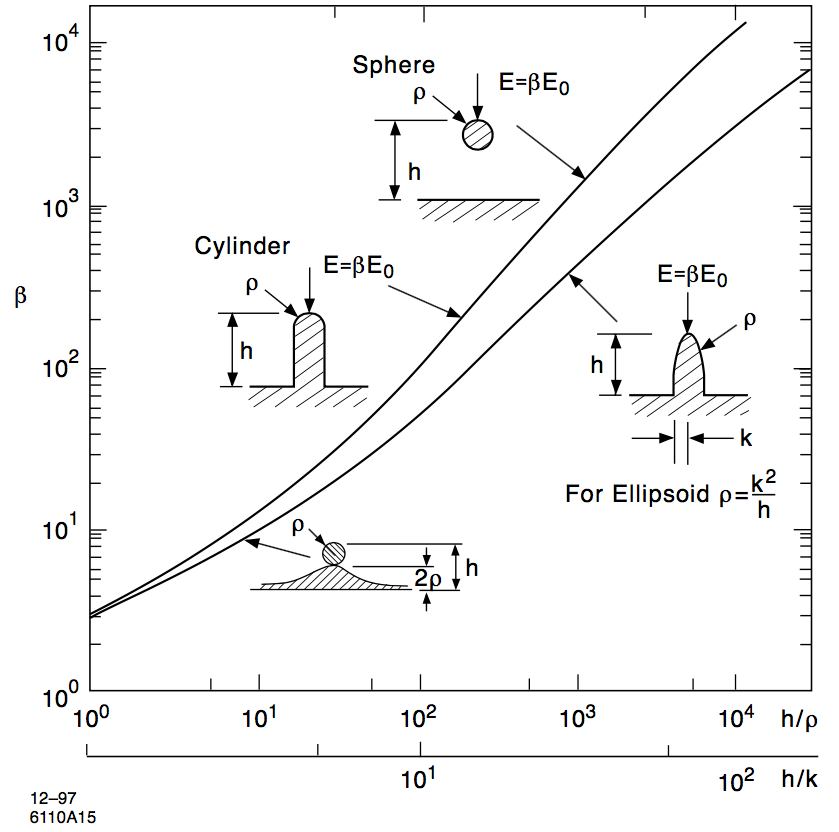
\includegraphics[scale=0.3]{pictures/beta_tip_val}
\caption{Field enhancement factors for simple geometries of metallic protrusions, plotted as function of geometrical features. From \cite{Rohrbach:190223}}
\label{tip_factors}

\end{figure}


%%%%%% EXCURSUS ABOUT REASONABLE VALUES OF BETA




\subsection[High power limits]{High power limits}

In an historical perspective, the Kilpatrick's Critereon was the first attempt to create a high power limit for the vacuum breakdown valid both in DC and RF applications \cite{KilpLimit}. The model was based on the acknowledgement of the Field Emission, and suggesting that the vacuum arc was created by the cascade of secondary electrons ejected from the surface by ion bombardment. The main result was to find a law ruling the maximum electric field achievable without triggering a breakdown. 

This critereon was reviewed many times up to now, because the experiments conducted nowadays show a field limit 7-8 times higher than Kilpatrick's prediction, and this can be addressed to different reasons: first of all the quality of the machining of the structures has increased considerably since the 1950's; in second instance the condition inside the RF cavities are more complicated because of the particular geometry.

At the end of the 1980's J.D.Wang finally proposed a model based on microprotrusion effect on the field and field emission, that involves the formation of a micro-plasma during the breakdown process. Also the Kilpatrick's limit was revised again in order to match the experimental results. \cite{Wang:1986, kilp:story}

Furthermore theories on the mechanism of breakdowns evolved, and will be mentioned in chapter 3.

Without entering in the physics of the breakdown phenomenon yet, the two following scaling laws are currently used in the design of modern accelerating structures.

\subsection[Power flow based criteria]{Power flow based criteria}

Other scalings have been proposed, like the phenomenological $P/C$-criterion, where $P$ is the power flowing in the cavity and $C$ the minimum iris circumference. It is straightforward to see that this is strongly related to the maximum surface electrical field, which is stronger for smaller irises. It has to be underlined that this is suitable just to travelling wave structures (TWS), since the power flow in standing wave structures (SWS) is close to zero. 

In recent years a more advanced version of the scaling has been presented \cite{Wuensch:932674}, which is quantified by
\begin{equation}
\frac{P \tau^{1/3}}{C}
\end{equation}
where $P$ is the power flow through the structure, $\tau$ the pulse length and $C$ the minimum iris circumference. This has also been formulated as $(f \times P/C )^{0.5}$, which is a quantity linear with the field \cite{Wuensch:1004189}.

Anyway, although these criteria are still in use today for the accelerating structure design, finding a more general criterion valid for any type of cavity is necessary.

\subsection{The modified Poynting vector $S_c$}

During the development of high-gradient normal conducting accelerating structures for the CLIC project, a new field quantity was developed, the \textit{Modified Poynting Vector} $S_c$, that is suitable both for TWS and SWS. \cite{Grudiev:newLoc}

The formulation is based on two assumptions: the breakdown process is determined by the accumulation of the pulses rather than the single pulse and the possible triggers of the breakdown can be induced by many processes that will be discussed later and are not relevant for the scaling law derivation.

A number of effects have to be taken into account (a simple geometry is considered, a cylindrical protrusion surmounted by a hemispherical  cap): 

\subsubsection{Pulsed heating by field emission current}

it is known that the field emission gets enhanced by the presence of the protrusion as described before. In this case the field enhancement factor can be expressed as $\beta \simeq h/r$, where $h$ is the tip height and $r$ is the cap radius. So the tip will emit a current according to the Fowler-Nordheim law \ref{If}, causing in first approximation the heating of the tip due to the ohmic heating as shown in figure \ref{figure_S_c}. Assuming that the edge of the tip will be the most heated part, and using the heat conduction equation, it is possible to derive the emitted current to melt the tip, which is found to be approximately $36$ A/$\mu$m$^2$ for a tip of $1$  $\mu$m height and a pulse of $100$ ns. This is consistent with the findings in \cite{soviet:1983}. The $\beta$ factor can be then derived, which is approximately between 40 and 60 considering a surface electric field in case of breakdown between 200 and $300$ MV/m, according with the experimental results.

 \begin{figure}
 \centering
 \subfigure[Electric field distribution]
   {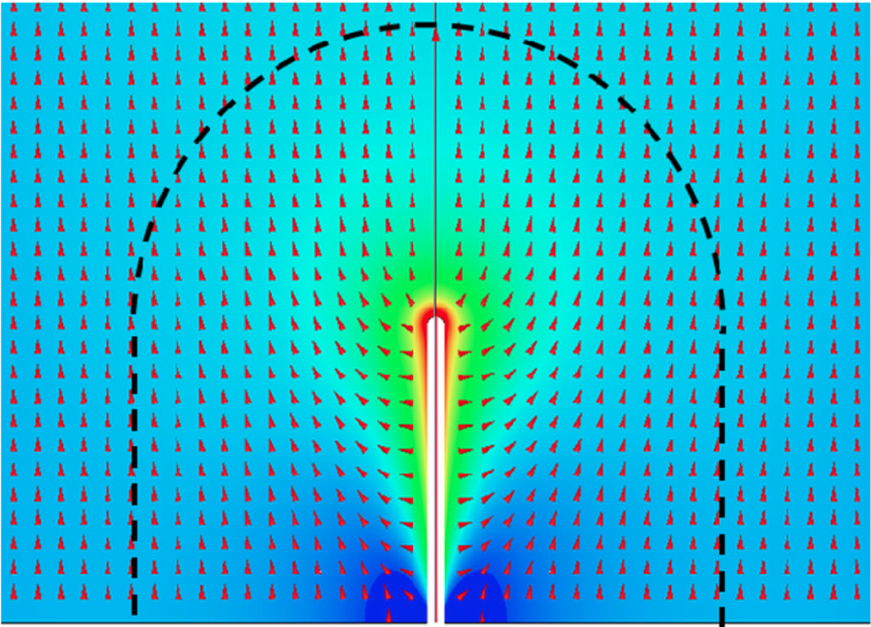
\includegraphics[width=6cm,height=5cm]{pictures/field_S_c}}
 \hspace{5mm}
 \subfigure[Field emitted power flow]
   {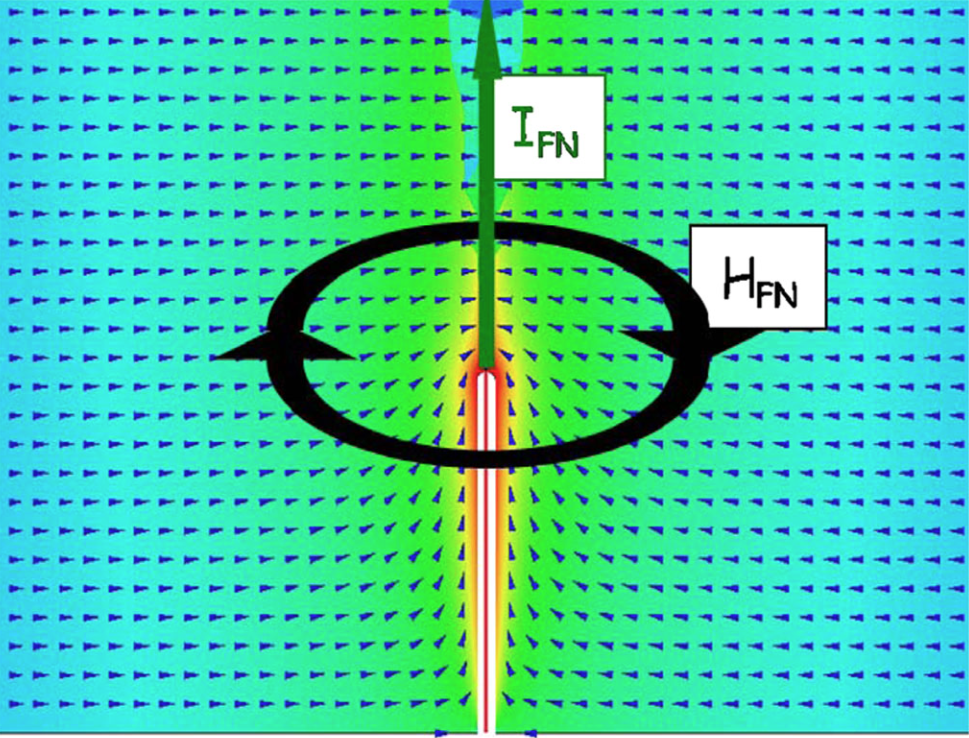
\includegraphics[width=6cm,height=5cm]{pictures/S_c_FEM}}
 \caption{(a) Electric field distribution around the protrusion considered. (b) Field emitted current and power flow. In both the plots arrows indicate the direction of the field and the color code the absolute value of the field, mapped logarithmically.\cite{Grudiev:newLoc} }
 \label{figure_S_c}
 
 \end{figure}



\subsubsection{Power flow near an emission site}

The heating of the tip mentioned before requires a huge amount of energy, which can be supplied only by the RF power present into the cavity. This is described by the Poynting vector $S_{RF} = E\times H_{RF}$. As discussed before a current is established in the tip, and flows through, subtracting energy to the EM field in the surroundings of the tip. The current flows through the tip and leave it at the edge, getting sprayed in the cavity according to the Fowler-Nordheim theory. Since any current flowing creates an associated magnetic field, the power flow due to the emission is given by $S_{FN}=E\times H_{FN}$. 

The key point is that since the copper is a very good conductor, to provoke a notable ohmic heating of the tip, a significant power flow through the tip is necessary. This can be calculated evaluating the $S_{FN}$ at a distance $d=h$ from the edge of the tip, where the electric field is not perturbed anymore by the shape of the tip itself. This can be formulated as the condition 
\begin{equation}
P_{RF} \ge P_{FN} \gg P_{loss}
\end{equation}
where $P_{loss}$ is the power lost for ohmic heating and $P_{FN}$ the power flow through the tip.

Considering now the relative phase of the $P_{RF}$ and of the $P_{FN}$ it is possible to derive an expression for the power emitted from the tip in a copper cavity
\begin{equation}
P_{FN} (t) = A \, E^3_0 \, sin^3 \omega t \,  \, exp \left ( \frac{-62}{\beta E_0 \, sin \, \omega t} \right )
\end{equation}
where the work function of the copper $\phi = 4.5 \, eV$ has been used, $A$ is the area of the conductor and $\omega = 2 \pi f$ is the angular velocity.

The RF power can be divided in real and imaginary part, with a phase shift of $90^\circ$. The real part is the energy propagating into the structure only and the imaginary part is the energy stored in the cavity both magnetically or electrically as it is the case in every resonant cavity. Since the active power flow is more efficient than the reactive one in providing power for the field emission, a weighting factor $g_c$ is introduced. The values of $g_c$ are slowly as function of the local electric field. For practical reasons all the simulation codes work using the complex Poynting vector $\bar{S}$, the precedent reasoning can be adapted to follow this practice, using the \textit{Modified Poynting Vector}
\begin{equation}
S_c = Re\{ \bar{S} \} + g_c \, Im \{ \bar{S} \} \qquad [W/\mu m^2]
\end{equation} 

Since this quantity can be calculated in any point of a structure, this allows to identify in advance the regions which are more sensible to the breakdown process. The rule of thumb given by the experience says that this quantity should not exceed the value of $5$ W/$\mu$ m$^2$ to have a breakdown rate smaller than $1\times 10^{-6} $ bpp  m$^{-1}$ with a pulse length of $200$ ns.

This quantity has been used to design all the lateset generations of CLIC structures, including the one tested in this work.






\section[The TD26CC structure for the Main Beam of CLIC]{The TD26CC structure for the Main Beam of CLIC}

After the precedent part about the general laws that regulate the operation of the TWS, now the structure under test in this work, the TD26CC, will be presented. The name stays for Tapered, Damped, 26-cells active cells structure with Compact Couplers.

It is necessary to keep in mind that in the design of the real cavities, it is almost never possible to use the general laws described in precedence because of the high complexity of the geometry. A great work of design and simulation is necessary, and is carried out with complex numerical simulations. This section will present a summary of the parameters and features of the cavity, the details can be found in \cite{CLIC:cdr,Grudiev:td26cc,Lunin:1333709}.

As pointed out in \cite{CLIC:cdr}, the main constraints in the structures for the main beam linac are 
\begin{enumerate}
\item Maximum surface electric field: $E_{surf}^{max} < 260$ MV/m
\item Pulsed surface heating: $\Delta T^{max} < 56$ K
\item Power density: $P_{in}/C\tau_p^{1/3} < 18$ MW/mm ns$^{1/3}$
\end{enumerate}

These limitations, together with the parameters listed in section 1.2.2, lead to the current design after a careful optimisation and tradeoff of the parameters. The main parameters are reported in Table \ref{TD26_param_1}

\begin{table}[h]
  \centering
    \begin{tabular}{ l l  }
    \hline
    \hline
    Average loaded accelerating gradient			& $100$ MV/m	\\
    Frequency								& $12$ GHz	\\        
    RF phase advance per cell					& $2/3 \, \pi $ rad	\\       
    Average iris radius to wavelength ratio			& $0.11$	\\ 
    Input, output iris radii      					& $3.15, \, 2.35 $ mm	\\
    Input, output iris thickness      				& $1.67, \, 1.00 $ mm	\\
    Input, output group velocity					& $1.65, \, 0.83 \, \% \text{ of c} $	\\
    First, last cell Q-factor						& $5536,\,5738$\\
    First, last cell shunt impedance				& $81,\,103 $ M$\Omega$ / m\\
    Number of regular cells						& $26$	\\   
    Structure length including couplers			& $230 $ mm	\\   
    Filling time								& $67 $ ns	\\               
    Total pulse length							& $242 $ ns	\\      
    Peak input power 							& $61.3 $ MW	\\        
    RF-to-beam efficiency						& $27.7 \, \%$	\\   
    Maximum surface electric field				& $230 $ MV/m	\\           
    Maximum pulsed surface heating				& $47 $ K	\\       
    \hline
    \hline
    \end{tabular}
  \caption{Parameters of the structure}
\label{TD26_param_1}
\end{table}

 \begin{figure}[h]
 \centering
 \subfigure[A disk composing the structure]
   {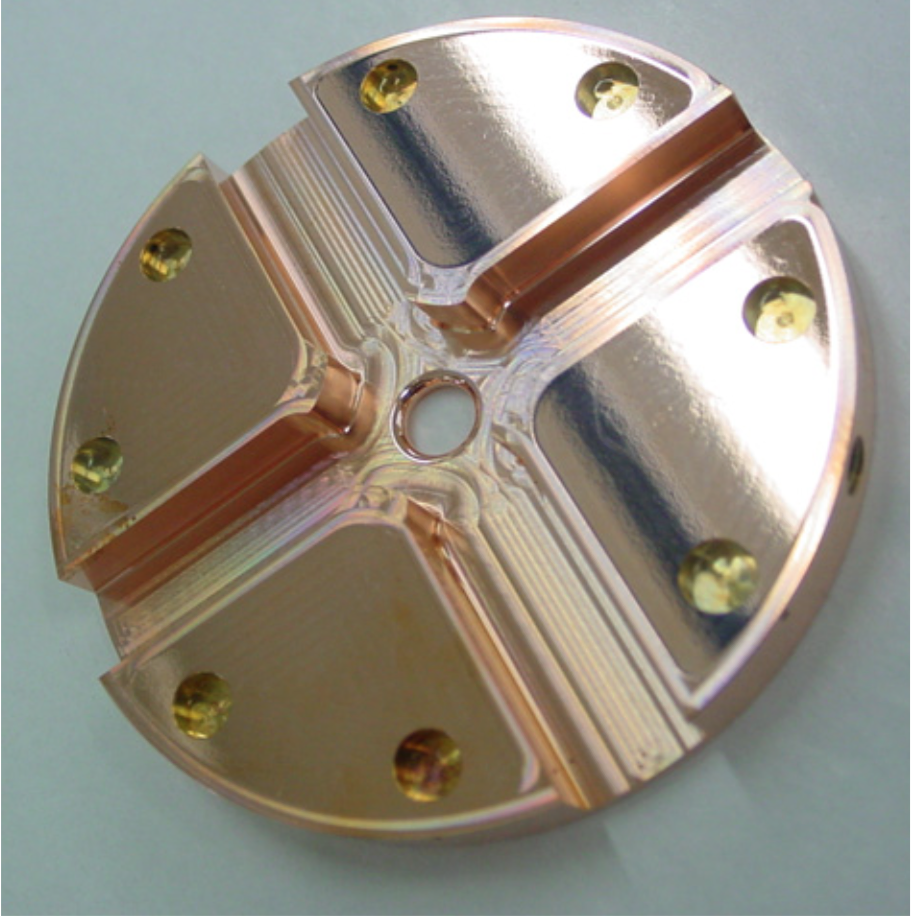
\includegraphics[scale=0.16]{pictures/photo_disk}}
 \hspace{5mm}
 \subfigure[CAD model of the structure, open to show the damping material]
   {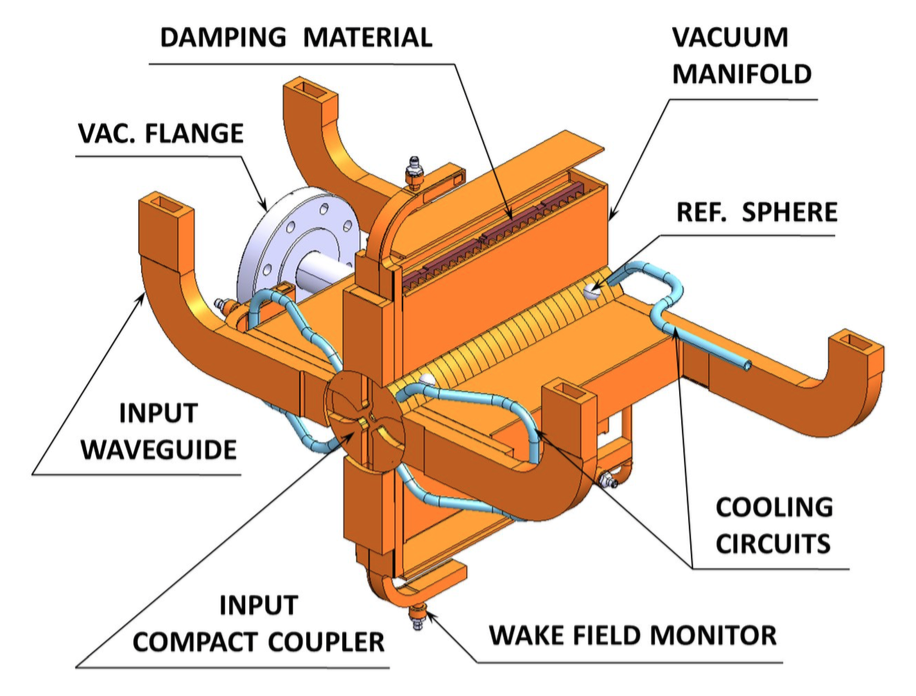
\includegraphics[scale=0.22]{pictures/TD26_layout}}
 \caption{A disk composing the structure (left) and the scheme of an accelerating structure (right), including couplers for the RF, cooling elements and connection flanges. The wakefield monitor is not present in the prototype under test}
 \label{CLICdisk}
 
 \end{figure}
 
The structure is fabricated stacking machined copper disks that are brazed together with a particular procedure that has been elaborated in order to achieve the highest mechanical precision possible in the alignment of the parts. Figure \ref{CLICdisk} shows a disk and a model of the accelerating structure.

The iris radius and thickness are linearly tapered in order to optimise the various high power parameters and to create a smooth field profile along the structure. 

Because of the high number of bunches per train and of the very short spacing between them (see table 1.1), the structure is realised in order to extract the transverse wakefields that can develop in the structure. This is realised using 4 symmetrical waveguides of dimensions carefully selected in order to allow the propagation of just the higher order electromagnetic modes (HOMs) but not the fundamental one that is used to accelerate the bunches and is provided from the input couplers. Once extracted, the transverse wakefields are damped on tips of Silicon Carbide (SiC) that are placed 50 mm away from the axis of the cavity.
The tapering also provides detuning of the high order modes, which are an issue even for highly damped structures.

Cooling water circuits and the vacuum flange are also installed the structure. The "CC" in the initials of the cavity name refers in fact to the particular shape of the coupling cells of this structure.

\begin{figure}[h]
\centering

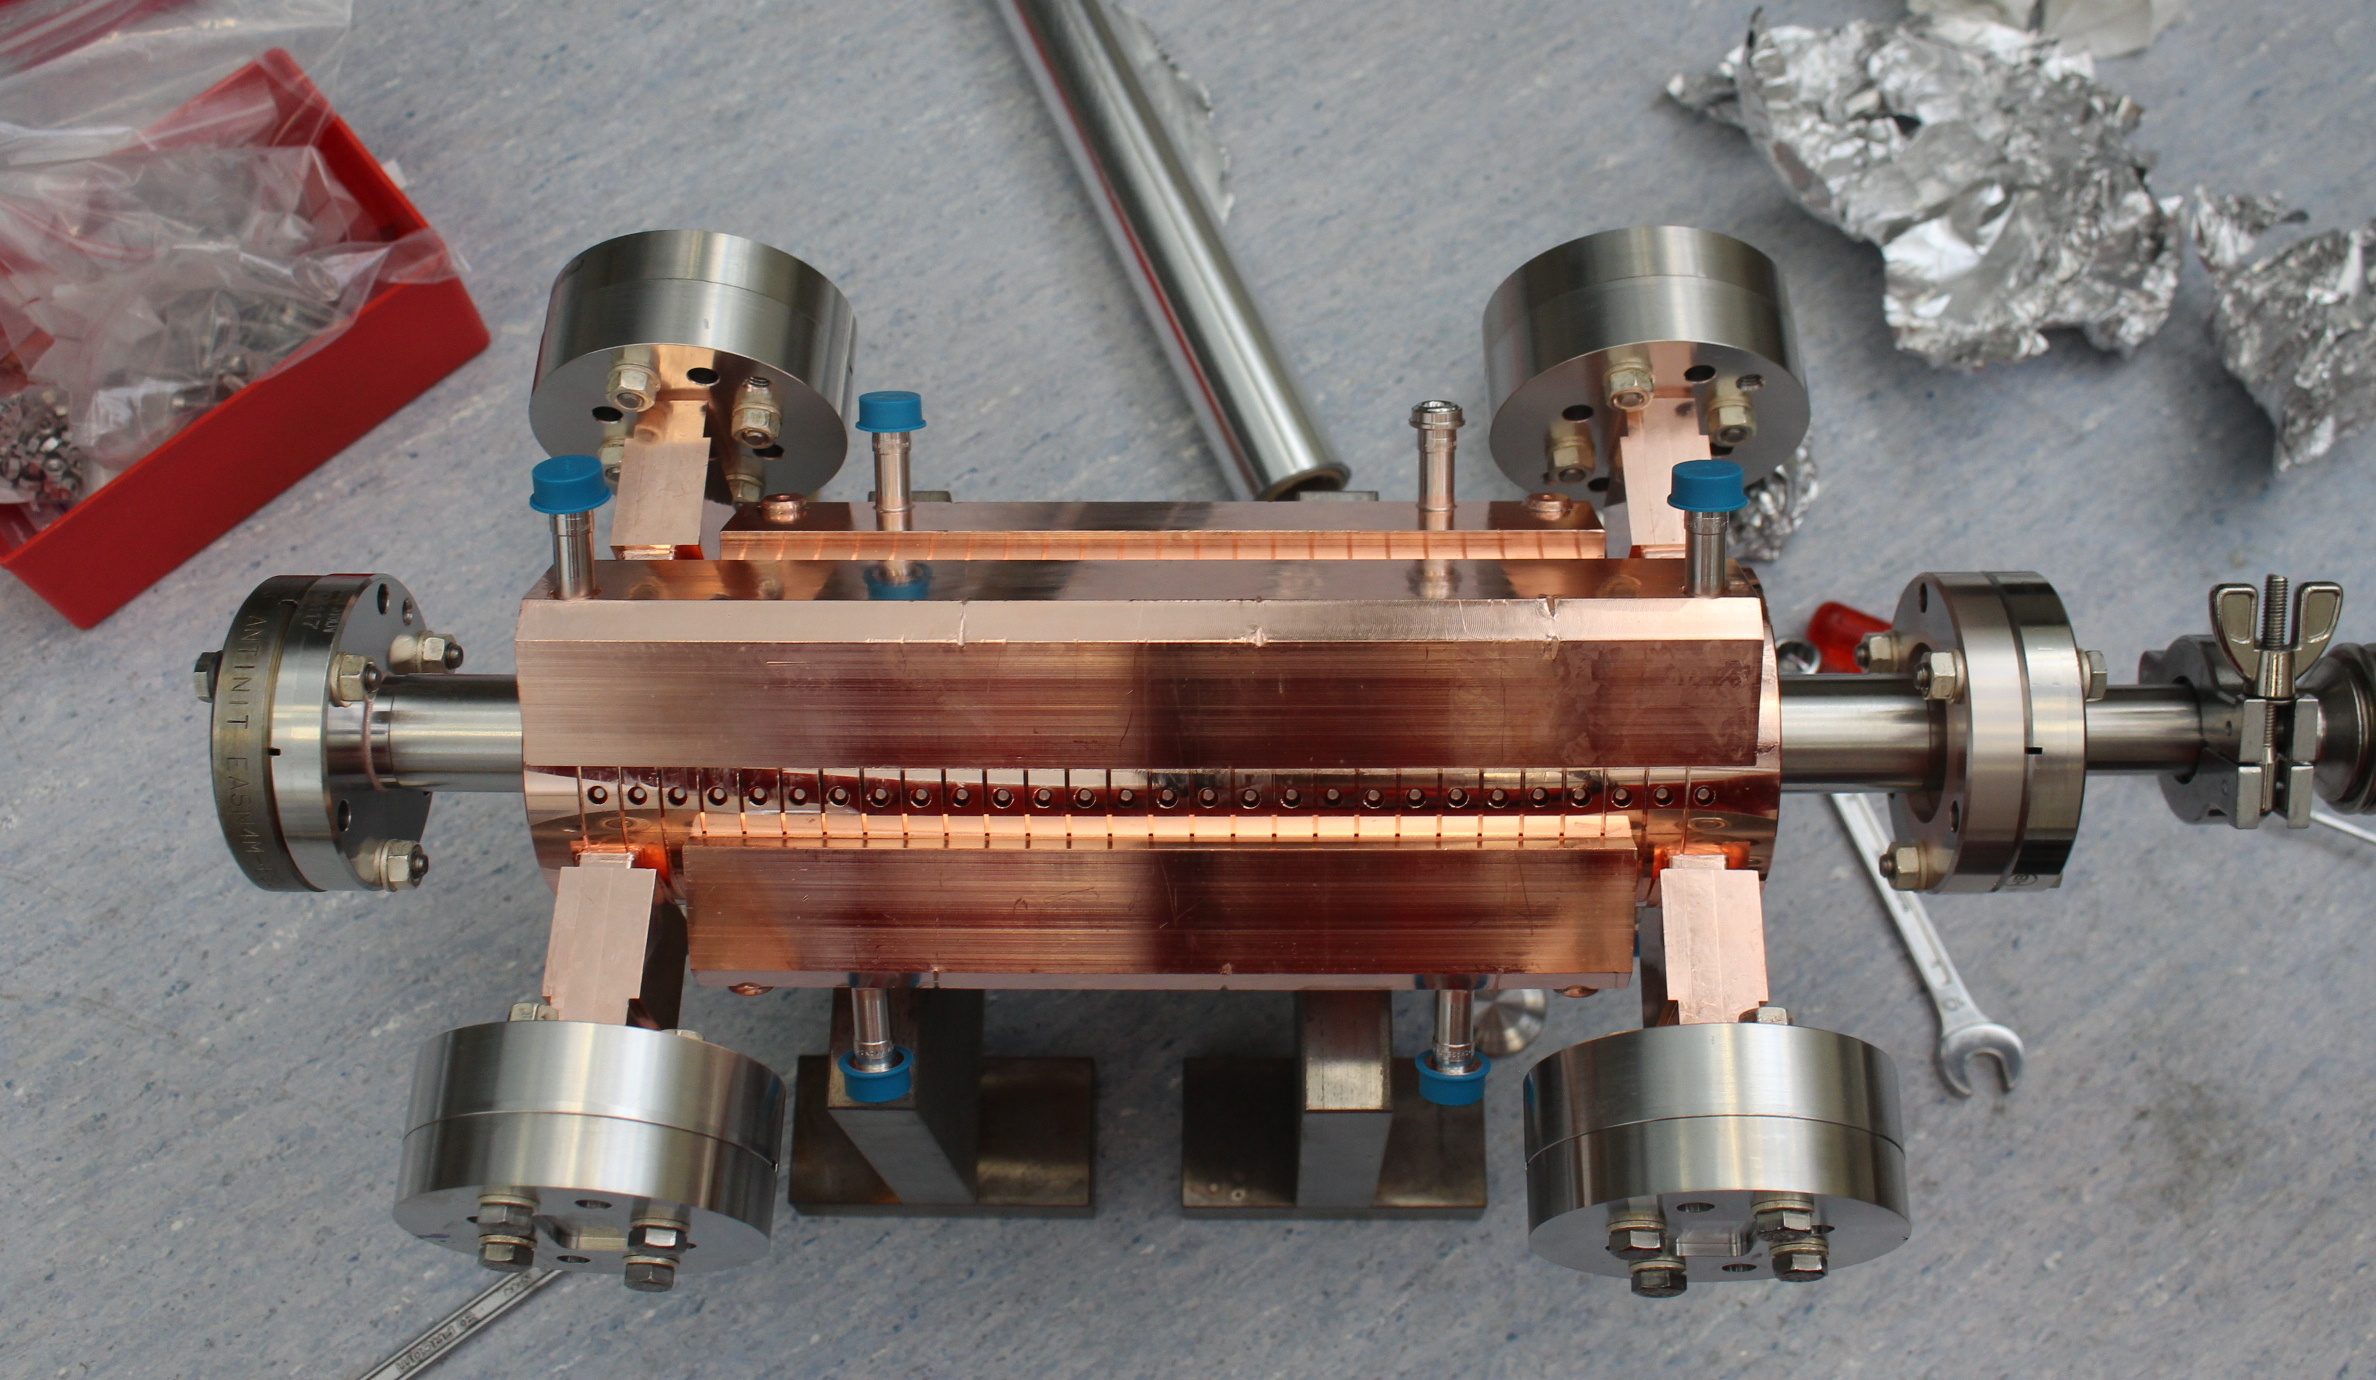
\includegraphics[scale=0.16]{pictures/td26_test_photo}
\caption{The structure prototype before the installation \textit{(Photo A. Solodko)}}
\label{td26_test_photo}

\end{figure}



\clearemptydoublepage
\chapter[The breakdown process]{The breakdown process}

This chapter will present the detected effects of the breakdowns and some topics about the physics. Typical setups for studies of vacuum arc physics will not be presented indeed, and a good summary can be found in \cite{Kovermann:1330346}. The reason is that the setup used in this work just gives the possibility to have a glimpse on the beam effect, but not to perform the measurements that are normally carried out in breakdown physics. This is caused by the beam presence, that makes the majority of the necessary sensors blind or not installable.

The large amount of parameters that play a role in the breakdown process makes researching in this field very complicated. For the same reason it is also very difficult to compare different experiments. This situation has led to a division in the scientific community about the theoretical description of the phenomenon.

Researchers anyway converge on the fact that, in high vacuum condition, the vacuum arc initiation process is dependent by the surface and material properties, but is independent from the pressure itself \cite{alpert:triggers}.

Strong efforts in pursuing the understanding of the phenomenon have been made so far, resulting in the improvement of the maximum gradient achievable in accelerating structures and the development of the first simulation codes~\cite{Insepov:1373092}.



\section[Detected effects of breakdowns in accelerating cavities]{Detected effects of breakdowns in accelerating cavities}

Most of the theories about breakdown converge on the fact that the breakdown and the field emission are different phenomena. While the field emission is always present, the breakdown of the field is a rare event, and depends by different causes, first of all the material.

Therefore in the detection of the breakdown a background current emitted by field emission is always present, but on top of that are notable during the breakdown \cite{Wuensch:583549}:

\begin{itemize}
\item RF pulse reflection: after the breakdown the incoming power is reflected back
\item An isotropical emission of X-rays. Unfortunately passing through the structure any information carried by the spectrum is lost
\item Visible light emitted by the arc
\item Current bursts exiting the cavity
\item Vacuum level spikes: this effect fades while the conditioning continues. This will be discussed in the section~\ref{sec:conditioning} 
\end{itemize}
Other effects, such as shock waves, have also been observed \cite{Rajamaki:2143815}. 

Figure \ref{RFandBPM} shows an RF pulse and the current burst measured with the setup used in this work during a run without beam. The fall of the transmitted power and the raise of the reflected one are clearly visible. Comparing the area of the two signals to the previous pulse, it is clear that a significant amount of energy is missing. This is normally attributed to the large amount of energy necessary to sustain the plasma that forms during the breakdown. The current burst emitted by the cavity on the downstream beam position monitor (BPM) is visible qualitatively on the right. It has to be kept in mind that the BPM is placed far from the exit of the cavity, resulting in a poor charge detection because of the small solid angle covered. Also the proper device to collect the emitted charge is a Faraday Cup, which cannot be installed in this setup because would obstruct the beam pipe. 


\begin{figure}[h]
\centering
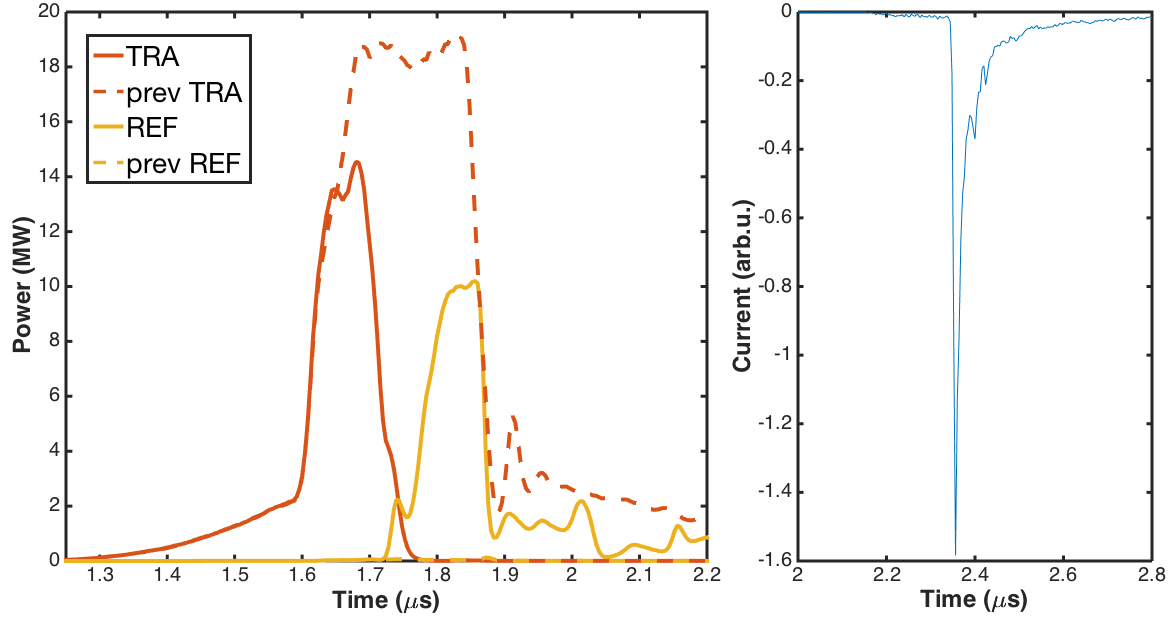
\includegraphics[scale=0.33]{pictures/RFandBPM.png}
\caption{RF signals of a breakdown event (left) and burst of current emitted, detected by a BPM (right). The left plot shows the fall of the transmitted power (solid red) and the raise of the reflected power (solid yellow). The RF signals of the previous pulse, so without breakdown, are reported dashed. Note that the time scale in the two plots are not comparable.}
\label{RFandBPM}
\end{figure}




\section[Vacuum arc process description]{Vacuum arc process description}

A fully satisfactory theory to describe the breakdowns has not been formulated yet, but the scientific community produced a number of models to describe the breakdown mechanism and initiation, summarised in \cite{soviet:1983,davies:triggers}. Most of them converge on the role that the field emission would have in triggering the breakdown, even if irrefutable  evidences have to be shown yet.

\subsubsection[Triggers]{Triggers}

The surface of the cathode is not completely flat, but presents some roughness that enhances the field emission as pointed out in chapter 2. This process leads to the formation of hot zones called \textit{field emitters} where the local electric field is enhanced by a factor $\beta$ because of the geometry and the current emitted is therefore increased (see Fig. \ref{BD_rocess}, box a). 

The current flow through the tip heats it up, modifying its physical properties and applying a tensile stress. Theories diverge on the process that takes place at this point: some are inclined to the heating up of the tip up to the fusion, like \cite{Grudiev:newLoc}; others on the cracking process of the tip due to the tensile stress applied by the enhanced electric field, which gets comparable to the tensile strength of the material around fields of $10$ GV/m  \cite{Insepov:1373092}.

It is in any case possible that during this process the shape of the tip gets modified, enhancing the $\beta$ factor even more.


\subsubsection[Plasma initiation]{Plasma initiation}

The peculiarity of the breakdown is that is a phenomenon that takes place in vacuum, and has been detected even at large gaps. According to many experimental results, the plasma is created from the cathode material (regardless on how it got emitted from the surface). The cathode material forms a neutral gas surrounding the tip, that gets ionised by the electrons emitted by field emission (see Fig. \ref{BD_rocess}, box b). In this first phase the ions created in this manner drift under the effect of the space-charge effect. The plasma initiation last only few ns.

Spectroscopical measurements of the light emitted by the plasma have shown that the plasma is formed of ions with various charge and electrons. The DC spark system at CERN showed that the plasma formed by copper cathodes present ionisation levels up to Cu$^{3+}$ \cite{Kovermann:1330346}.


\subsubsection[Plasma evolution]{Plasma evolution}

The ion density of the plasma over the emitter results in the establishment of a sheath potential, which enhances the electrical field even more, provoking an exponential  increase of the field-emitted current. The current emitted reaches values of several A/$\mu$m$^2$, resulting in the melting of the emitter (see Fig. \ref{BD_rocess}, box c).

The molten metal becomes part of the plasma, that expands modifying temperature and density. The sheath potential gets modified as well. After an expansion process, where part of the plasma interacts with the surface, determining erosion, the greatest part of the ions recombinate with the electrons determining an intense optical emission.


\subsubsection[Cratering phase]{Cratering phase}

During the last plasma expansion, the ions impacting on the surface are expected to create new field emitters. The emitters will melt and result in an explosive emission because of the high field provoked by the sheath potential (see Fig. \ref{BD_rocess}, box d). 

The full arc is expected to continue up to the end of the RF pulse. Next the plasma is expected to disappear due to expansion cooling or recombination. All the process results in a surface damage in the emitter zone and the surroundings. If in the damaged zone other protrusions have been created, they will trigger new breakdowns according to the new value of $\beta$ (see Fig. \ref{BD_rocess}, box e, f). 

Figure \ref{SEM_crater} shows a photograph of a crater, taken using a scanning emission microscope.
\begin{figure}[h]
\centering
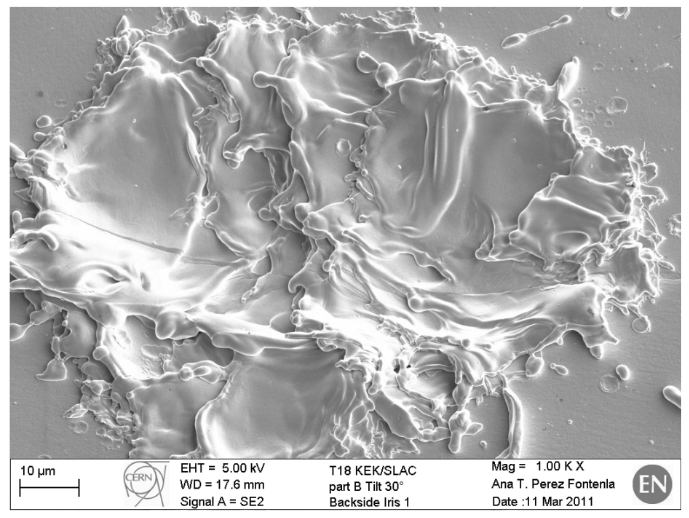
\includegraphics[scale=0.4]{pictures/crater}
\caption{Crater provoked by a breakdown in an X-band RF accelerating cavity \cite{Wuensch:advaces}}
\label{SEM_crater}
\end{figure}



\begin{figure}[h]
\centering
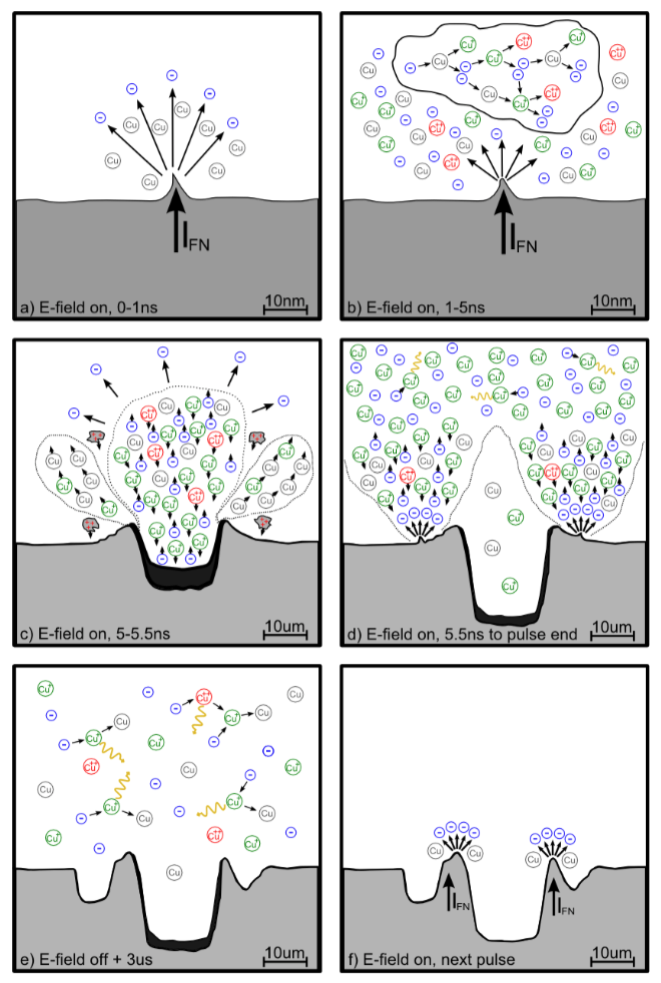
\includegraphics[scale=0.4]{pictures/BD_process}
\caption{Breakdown stages in chronological order. From \cite{Kovermann:1330346}}
\label{BD_rocess}
\end{figure}


\section[Breakdown rate scaling law]{Breakdown rate scaling law}

The interest on breakdowns in accelerator physics arose in order to avoid as much as possible perturbations of the beam. This materialises mainly in kicks to the beam passing through the plasma \cite{Palaia:1625826}, and change of the acceleration because the reflection of the RF power modifies the field distribution inside the accelerating cavities.

 A key parameter of an accelerating cavity is the breakdown rate (BDR). The breakdown rate is the number of breakdowns that happens per number of RF pulses. Measuring the BDR of a cavity means to measure a probability, and requires to accumulate a sufficient number of pulses. 

According to the latest developments, the BDR follows the scaling law
\begin{equation}
BDR \propto E^{30}_a \tau^5_p 
\label{E30}
\end{equation}
where E$^{30}_a$ is the cavity accelerating gradient, and $\tau_p$ the pulse length  \cite{Wuensch:advaces}.

This scaling law allows to compare the performance of different accelerating structures and different tests. It is important to underline that the scaling law was deduced by the results of the experiments executed so far, but does not imply any kind of assumption on the physics of the breakdown process.




\section[Influence of the conditioning process]{Influence of the conditioning process}
\label{sec:conditioning}

It has been mentioned how the trigger mechanism of the breakdowns seems to depend on the condition of the surface of the accelerating cavity. In order to reach the low breakdown rate that is required for the performance of the linear colliders, two strategies have been used:
\begin{enumerate}
\item Refining of the production and assembly techniques of the cavities
\item Conditioning the structure with a series of RF pulses increasing the power gradually and keeping the breakdown rate limited
\end{enumerate}
The current production procedure for the structures for CLIC is outlined in~\cite{CLIC:cdr}. The conditioning process is a more complicated matter. 

The conditioning of an accelerating structure is conducted applying repeatedly RF power pulses at a fixed pulse length, while keeping the breakdown rate limited under a certain threshold. This is realised modifying the input power, that gets raised after a period without breakdown, or lowered if the breakdown rate gets too high. When the power goal has been reached, the pulse length is increased, and the process restarts with low power pulses.

The process terminates when both the power and the pulse length goal has been reached. In many experiments the breakdown rate has exhibited an exponential decrease with the conditioning time. The conditioning of a structure may last up to 3-4 months to reach the design breakdown rate. Understanding the process and finding the right conditioning strategy becomes important, and many efforts have been made in this sense. The surprising result is that the conditioning process proceeds with the number of RF pulses rather than the number of breakdowns happened \cite{Degiovanni:2065711}.

The physical process that provokes breakdown might change as long as the conditioning goes on. According to recent results \cite{Wuensch:583549}, the vacuum level increase, that takes place during a breakdown, fades as time goes by. This effect is probably addressable to the stimulated desorbtion \cite{soviet:1983}, that provokes a gradual release of the absorbed gas into the metal, that gets pumped out. This effect is triggered in presence of strong electric fields only, the same fields that are involved during the breakdown process. The contribution of the desorbed gas is still not clear anyway. Another possible effect is the presence of dust particles on the surface, that gets cleaned up as conditioning continues.

A review of the conditioning algorithm used, and the conditioning history of the accelerating cavity used in this work can be found in \cite{Degiovanni:1742280}.











\clearemptydoublepage
\chapter[Experimental setup]{Experimental setup}
\label{chap:setup}

The high-gradient tests at CERN are carried out in the three X-band\footnote{The X-band is a segment of the electromagnetic spectrum in the region of the microwaves. The waves in this region have frequencies between 8.0 and 12.0 GHz.} test stands (XBOXs). These are setups able to provide the necessary high-power RF pulses to the structures under test. For the tests described in this work the presence of the beam inside the accelerating cavity is also necessary, and is provided by the electron linac of the CTF3. 


\section[Linac and dogleg]{Linac and Dogleg}

As mentioned in the first chapter, the main goal of the CTF3 is to demonstrate the feasibility of the CLIC acceleration scheme. For this reason, the linac is used to generate the Drive Beam pulse, that is sent to the rings for the recombination and then to the prototype Two-beam module. 

The linac is realised using conventional 3 GHz technology. The recombination process leads to the bunch frequency of 12 GHz. 

Given that the breakdown rate tests of high-gradient cavities was not in the initial design of the facility and differs from the standard operation, in the following sections only the part of the setup which is relevant for the breakdown experiments will be described. The full CTF3 accelerator complex is widely described elsewhere \cite{CLIC:cdr,CTF:drive_beam,ctf3:dr}. 

To perform high-gradient structure tests, a beam line parallel to the linac has been used. The two beam lines are connected by an oblique segment, resulting in the characteristic shape that is the origin of the name \textit{Dogleg}.

For the high-gradient testing purpose the accelerator  simulates the CLIC Main Beam. The parameters of the beam are reported in the Table~\ref{beam_par_dogleg}


\begin{table}
  \centering
    \begin{tabular}{ c l }
    \hline
    \hline
    Current 		&	$1.6$ A\\
    Pulse length		&	$250$ ns\\
    Energy			&	$130$ MeV\\
    Reptition freq.	&	$0.83-25$ Hz\\
    \hline
    \hline
    \end{tabular}
\caption{Beam parameters used in the Dogleg \cite{NavarroQuirante:2025954}}
\label{beam_par_dogleg}
\end{table}



\subsubsection{Injector}

The production of the beam is realised by a 140-kV thermoionic gun, designed to deliver up to $5\,A$ of current in nominal operation conditions.
The gun is followed by a S-band\footnote{The S-band is the segment of the electromagnetic spectrum in the region of the microwaves. The waves in this region have frequencies between 2.0 and 4.0 GHz.} prebuncher and a 17 cell travelling-wave buncher. These structures are followed by two 1.2-m long accelerating structures. The beam dimension in this initial phase is controlled by means of solenoids, up to the second accelerating structure \cite{ctf:injector}.

Downstream of the injector a magnetic chicane with collimators is installed to eliminate off-energy particles and to perform bunch compression  \cite{Braun:999488}.

The layout of injector and chicane are reported in Fig.~\ref{injlayout}.

\subsubsection{Linac}

Three modules composed of two S-band accelerating structures operating at 3 GHz are installed in the linac. The accelerating structures consist of 32 regular cells, operating in the $2\pi/3$ mode. The damping of HOMs is guaranteed by radial slots in the iris, containing SiC loads. The structures are designed for fully loaded operation with a current of more than 4 A, but when simulating the Main Beam the current is significantly less, implying less loading. In this condition the energy gain is essentially bigger compared to Drive Beam operation.

The focusing is realised by triplets of quadrupoles, coupled with dipole correctors. The beam energy can be measured in the spectrometers in sector 4 and 10.

The layout of the linac is reported in Fig.~\ref{linaclayout}.

\subsubsection{The dogleg}

After sector 7 in the linac, another triplet of quadrupoles is located on the beamline, before a bending magnet. When the bending magnet is on, the beam is directed in the dogleg, passing through an oblique section, and is bent again to enter a segment of the beamline parallel to the linac. The optics of the dogleg beamline is designed to correct the dispersion provoked by the bending magnets. The structure under test is placed at the end of the dogleg line between two Beam Position Monitors (BPMs). Just before the structure there is a slit, in order to protect the coupling cell of the structure from being hit by a missteered beam. The beam is dumped downstream of the structure.

In case the first bending magnet is off, the beam proceeds straight in the linac, passing through a triplet of quadrupoles in section 9 and another triplet in sector 10. A spectrometer is placed after that, to measure the beam energy. 

The layout of the dogleg and of the linac up to section 10 is reported in Fig.~\ref{dolaut}.


\begin{landscape}
\begin{center}

\begin{figure}
\centering 
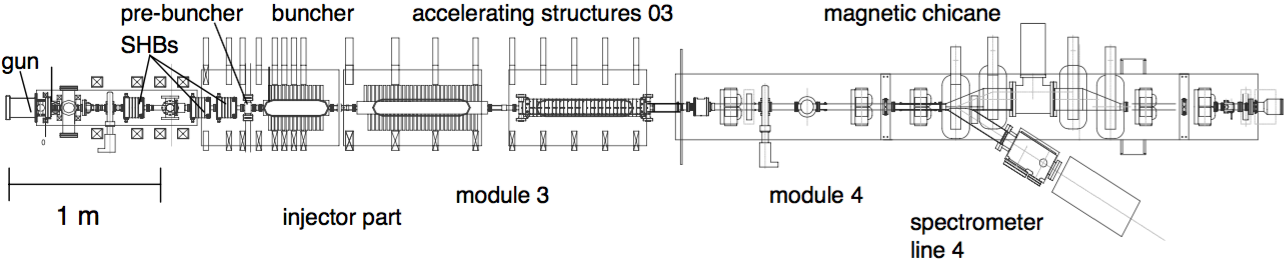
\includegraphics[width=23cm,keepaspectratio]{pictures/Injector}
\caption{Layout of the injector and the magnetic chicane. Legenda: SHBs: sub-harmonic bunchers.\vspace{4mm}}
\label{injlayout}
\end{figure}



\begin{figure}
\centering 
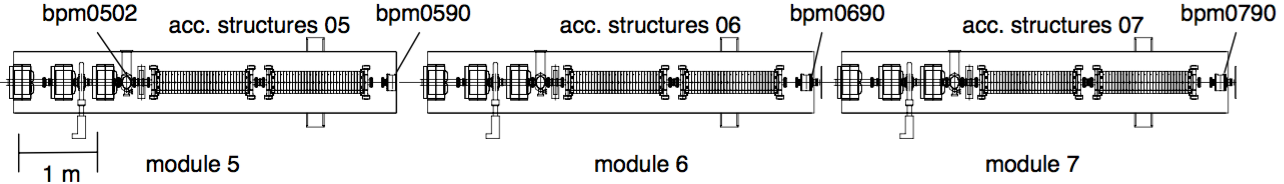
\includegraphics[width=23cm,keepaspectratio]{pictures/girder5-7}
\caption{Layout of the linac up to module 7. Legenda: bpm: beam position monitor.}
\label{linaclayout}
\end{figure}

\end{center}
\end{landscape}



\begin{landscape}
\begin{figure}
\centering 
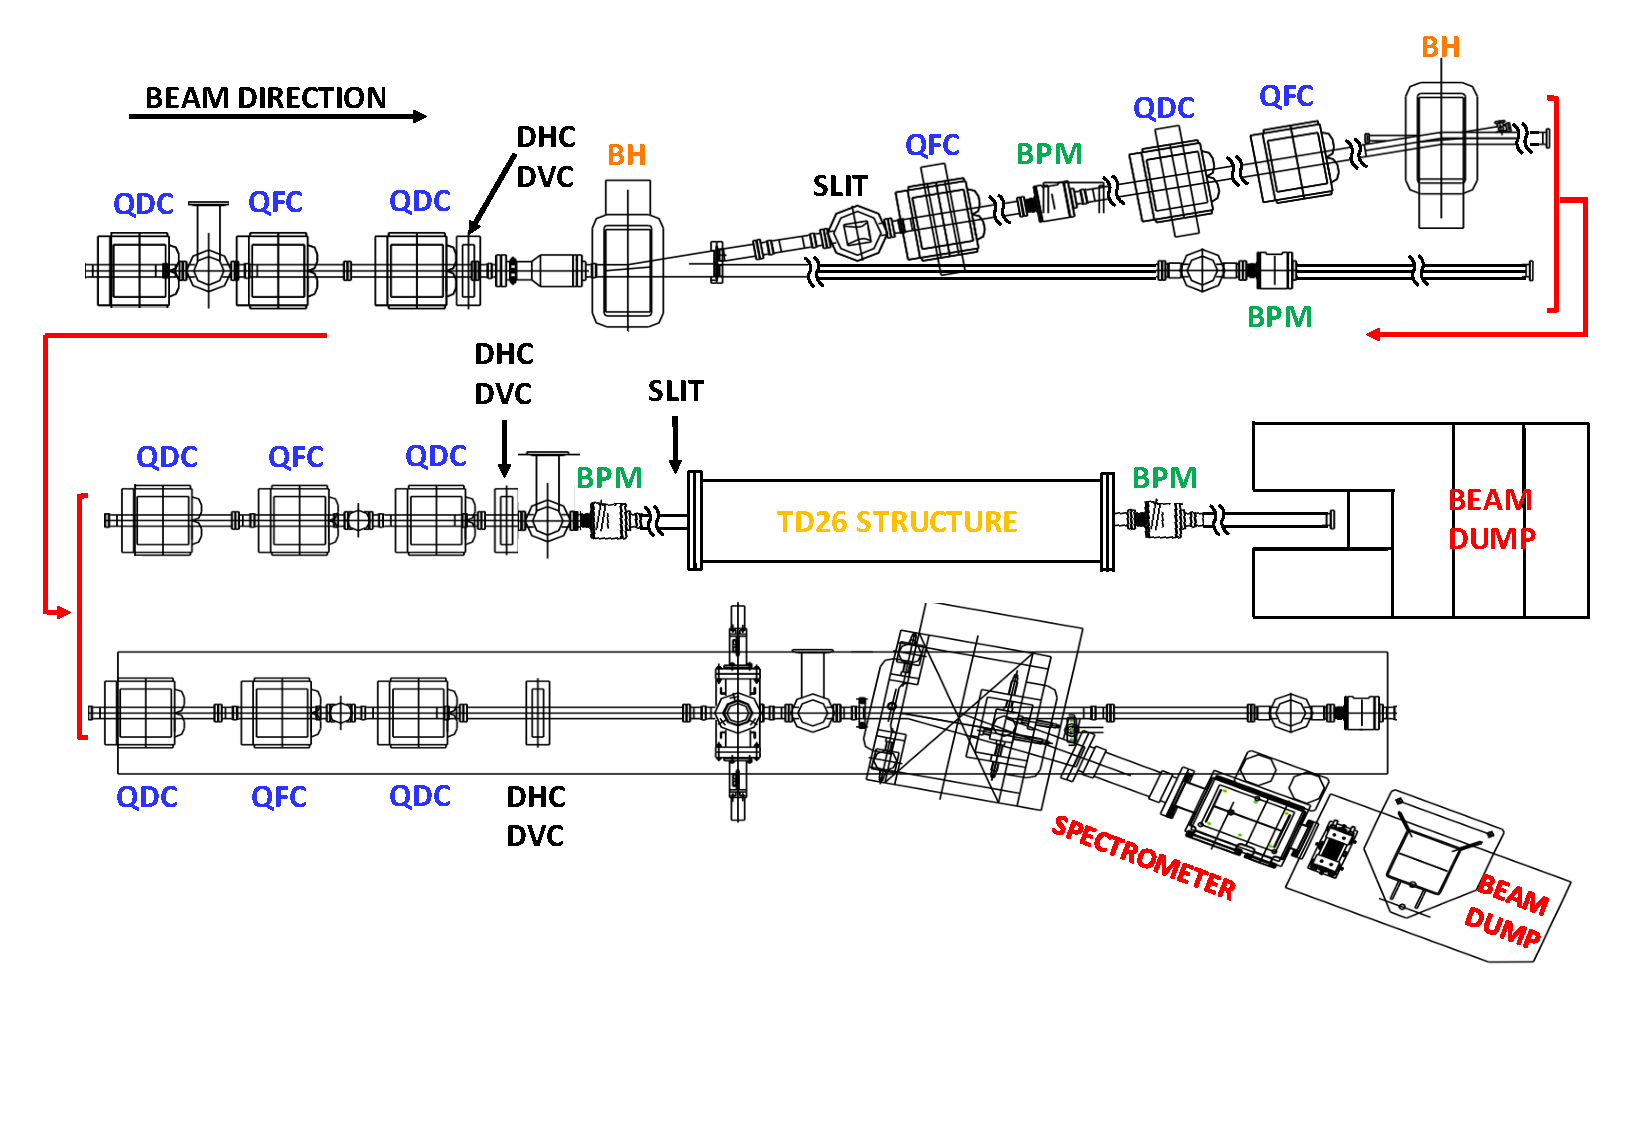
\includegraphics[scale=0.78]{pictures/modified_pets.pdf}
\caption{Simplified layout of optics and beam instrumentation of the dogleg line, adapted from technical drawings and facility layout \cite{EDMS:CTF3}. The beam for this section come from the end of the module 7. Legenda: QFC(QDC): focusing(defocusing) quadrupole; DHC(DVC): horizontal(vertical) dipole corrector; BH: bending magnet in horizontal plane; BPM: beam position monitor}
\label{dolaut}
\end{figure}
\end{landscape}



\section[RF power production]{RF power production}

The development of the accelerating cavity technology is strongly related to the possibility to produce and test prototypes. This test activity allows one to improve the understanding of the scaling laws of the phenomena that limit the performance of the accelerating structures, but also to compare the results of different production and conditioning techniques. 

At CERN the production of 12 GHz RF was once carried out only in the Two-beam modules in the CTF3. To enlarge the test capabilities standalone test stands were necessary. This was realised for the first time with the installation of the so called X-Band Test Stand 1 (XBOX1) \cite{Peauger:1287901}. Similar test stands are present in the Nextef facility at KEK and in the ASTA facility at SLAC. Currently there are three X-band test stands simultaneously active at CERN.

\begin{figure}[h]
\centering 
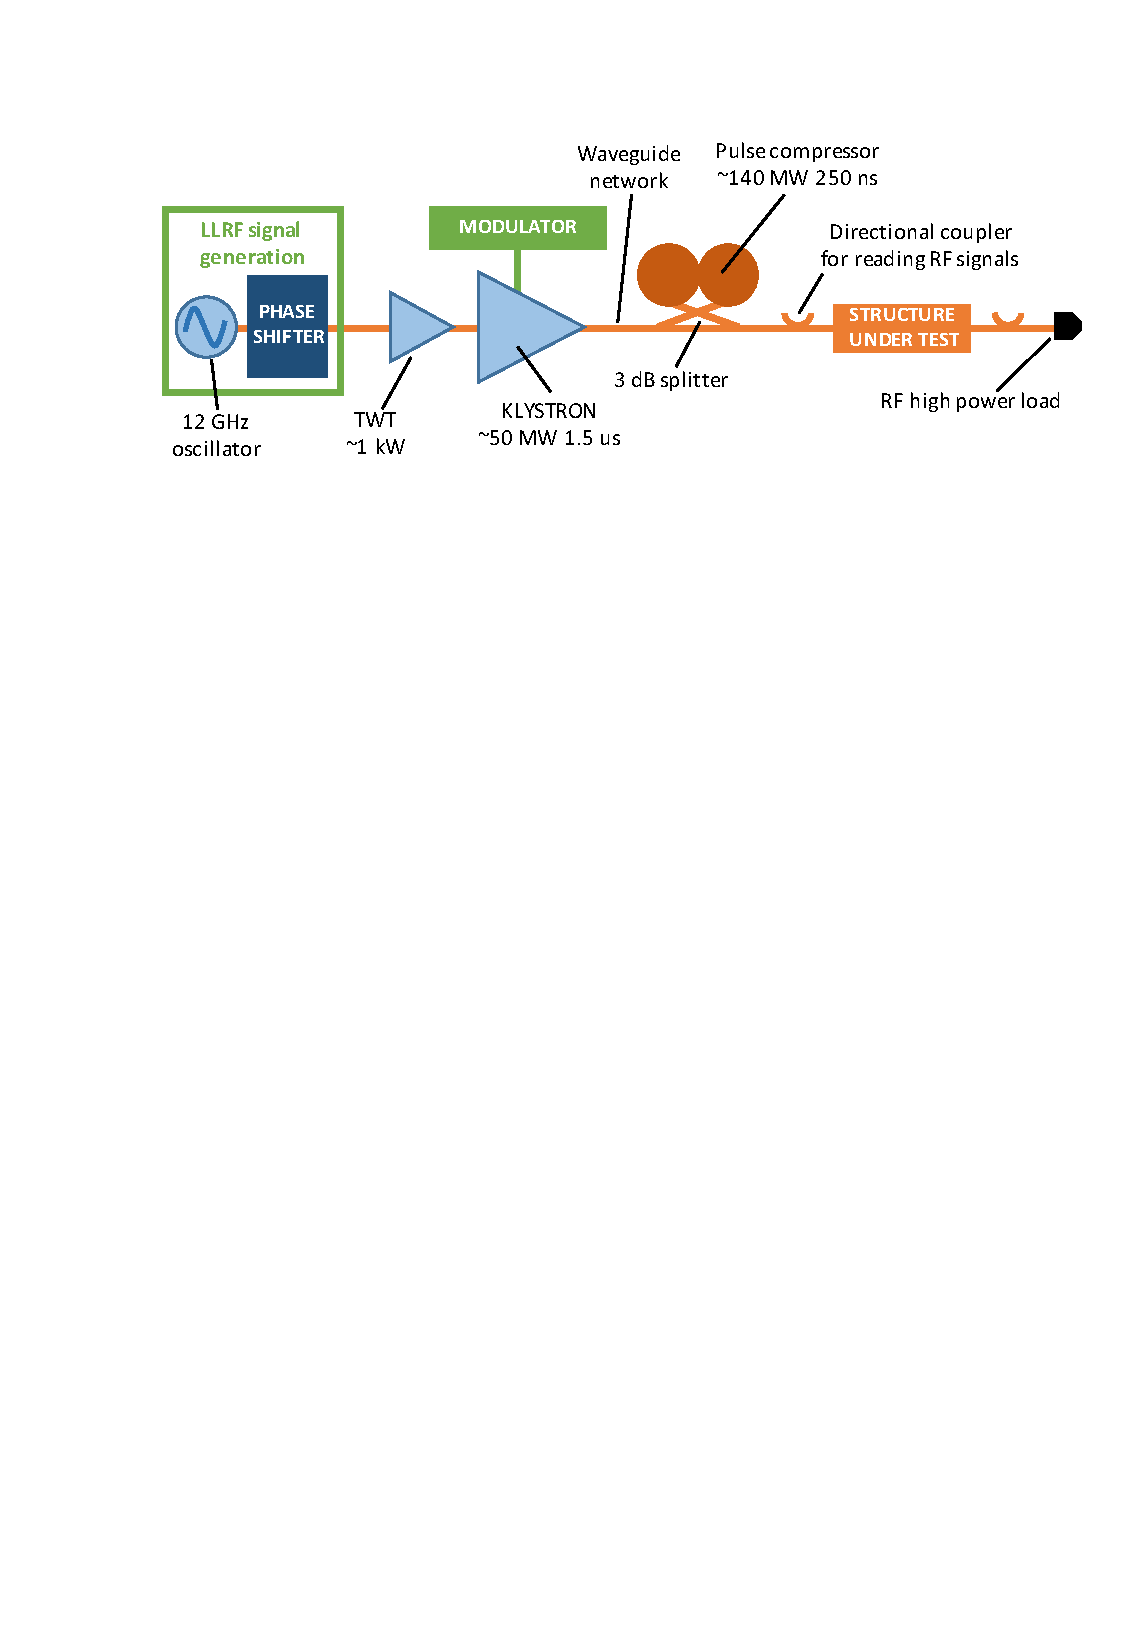
\includegraphics[scale=0.8]{pictures/test_stand_scheme.pdf}
\caption{Standalone X-band test stand layout}
\label{xbox_layout}
\end{figure}

The layout of a RF test stand is shown in Fig.~\ref{xbox_layout}. It is normally formed by signal generation, amplification and delivery systems; diagnostic and control systems, and service systems such as cooling and protection systems. 


\subsection[The X-Box1 at CERN]{The X-Box1 at CERN}

The proposal of an X-band test stand at CERN followed the change of the frequency of CLIC from 30 GHz to the european X-band 12 GHz in 2008. An organic description of XBOX1 is in \cite{Woolley:2015,Kovermann:1459879}. The high-power RF production is realised using:
\begin{itemize}
\item an XL-5 klystron, able to produce 50 MW of 12 GHz radiation with a pulse length of $1.5\, \mu$s and a repetition rate up to 50 Hz.
\item a Scandinova modulator, used to power the klystron.
\item a SLED-I type RF pulse compressor, able to compress the klystron output pulse to a shorter one of 140 MW, 250 ns long, which is sufficient to test accelerating structures considering the waveguide losses.
\end{itemize}

The RF delivery from the pulse compressor to the structure is realised using WR90 waveguides, kept under high-vacuum at a pressure of the order of\\ $5\times10^{-9}$ mbar. In order to reduce the losses, some part of the line to the structure under test is realised with low-loss waveguides. This structure requires mode converters because the fundamental modes of the waveguides are different. The overall transmission of the waveguide network has been measured to be around 67 \%.

More details regarding the key components of the system are presented in the following sections. The system is controlled solely by the Low-Level Radio Frequency (LLRF), since the gain of the amplification chain is fixed. This feature requires a unique control system of the LLRF together with the Data Acquisition system (DAQ), that will be described in section \ref{sec:RF_and_DAQ_s}.


\subsubsection{TWT, Klystron and modulator}

The very first power amplification stage is carried out by a Travelling Wave Tube (TWT) \cite{appSys:twt}, which is a device with the same working principle of the klystron (described below). It raises the power of the signal from some watts to up to 3 kW.

XL-5 klystrons comes from the effort made in SLAC to develop high efficiency klystrons for the Next Linear Collider project (NLC). They are based on the XL-4 klystrons, adapted from the american X-band frequency of 11.4~GHz to the european 12~GHz. This effort lead to the CPI VKX-8311A tubes that are currently in use \cite{klystron:CPI}, which are able to produce a pulse of 50 MW of power, $1.5 \, \mu$s long with an efficiency of the order of 40\%.
 
Klystrons are vacuum tube amplifiers. They are composed of a thermoionic gun, that emits a pulsed beam of electrons. The beam passes through one or several cavities, where a low power RF modulates the beam. After a drift space, where the beam is kept collimated by a solenoid and accelerated by a fixed DC field, the beam passes through a passive cavity that extracts the high power RF. The beam is then dumped. 

The klystron is operated in pulsed mode to reduce the wall-plug power consumption. This means that a power supply able to deliver short pulses of high power is necessary. XBOX1 uses a K-3 solid state modulator by Scandinova, able to supply voltage pulses up to 410 kV with currents of the order of 310~A.


\subsubsection{Pulse compressor}

The pulse compressor is the device used to convert the long pulse of the klystron into a shorter one at a higher power. The operation principle is that the power from the klystron is stored in high-Q resonant cavities during the pulse. Before the end of the pulse the cavities are emptied by reverting the phase of the input power. The emptying process is done in a shorter time than the filling time, determining the production of a short high power pulse. 

This technique can lead to peak power increase up to a factor 5-7. 

The SLED-I type pulse compressor is using two cavities, coupled with a 3~dB hybrid coupler, in order to discharge the produced power to the desired load instead of sending it back to the klystron. The theory behing the pulse compression is fully described in \cite{Fiebig:209756}, the application in XBOX1 in \cite{SLED:ctf3}.

The resonance frequency of the pulse compressor's cavities is strongly dependent on the volume, which depends on the temperature. For this reason the heat produced by the RF, due to the ohmic resistance of the walls, has to be disposed of by an external thermostatic system. An imperfect heat dissipation leads to the detuning of the cavities, which constitute an operational issue and will be extensively discussed later in section \ref{sec:xboxop} and \ref{sec:PCtune}.

 


\section[DAQ \& RF control systems]{DAQ \& RF control systems}
\label{sec:RF_and_DAQ_s}

The control system is in charge of generating a phase-modulated signal for the successive amplification stages (TWT and klystron). It also has to acquire the signals from the directional couplers, and the diagnostic signals from the structure and the vacuum systems. According to the diagnostic inputs, it modulates the signal and can also act on the beam permit of the gun of the linac. This last role is central, since the interlocking function is fundamental not only for the equipment protection, but also to trigger the data memorisation. 


\subsection[Hardware]{Hardware}

To perform his task, the control system is made of different components, including PLCs (Programmable Logic Controller) interlock systems,  VME (Versa Module Europa) crate based arbitrary signal generators, OASIS PC \cite{OASIS}-based digitisers and PXI (PCI eXtension Instrumentation)-based control systems.

The core of the system is the National Instrument PXI crate \cite{NI:PXI}, that is the most advanced system in the setup. It carries out the acquisition and processing of all the signals relevant for interlocking the system; triggers the interlocks; save in the internal memory the recorded signals and retrieves the signals sampled externally in case of an interesting event; interfaces with the rest of the instrumentation.

Since the phase of the LLRF signal has to be modulated to be able to perform the pulse compression, the LLRF signal is sent to an analog and a digital phase shifter in series. During the experiments with beam, the digital one is used to properly phase the RF with respect to the beam.

The data acquisition from the -50 dB directional couplers on the waveguides is performed using different kind of sensors:
\begin{enumerate}
\item Diodes with a bandwidth of 500MHz convert the RF signals to a DC voltage level
\item IQ\footnote{In-phase and quadrature components demodulators. These detectors measure amplitude and phase of an electromagnetic wave by mixing it to a known wave at the same frequency (in this case supplied by the main 12 GHz oscillator of the Xbox).} demodulators are used to measure the phase and the amplitude
\item Logarithmic detectors are used to acquire the signals with a wide dynamic range of over 46 dB
\end{enumerate}

The PXI crate has 8 channels of 14-bits, 250 MSa/s digitisers. These digitisers are connected internally to FPGAs in order perform the analysis as fast as possible, and send a signal to the trigger unit to interlock the LLRF signal production. A 24 channel Digital Multimeter (DMM) unit is used to read the vacuum signals from the ion pump controllers. The fast digitisers of the PXI acquire the signals from the logarithmic detectors. 

The signals of the IQ demodulators are sampled by OASIS acquisition PC containing 16 units of 1 GSa/s, 8-bits ADCs. These are read by the PXI crate for the breakdown events and archived for the offline analysis. 

The signals of the BPMs are acquired and recorded as well by one of the acquisition cards of the PXI crate.

Figure \ref{high_l_RF} shows schematically the high level RF described above and the acquisition equipment that is used for diagnostic and data analysis.

\begin{figure}[h]
\centering 
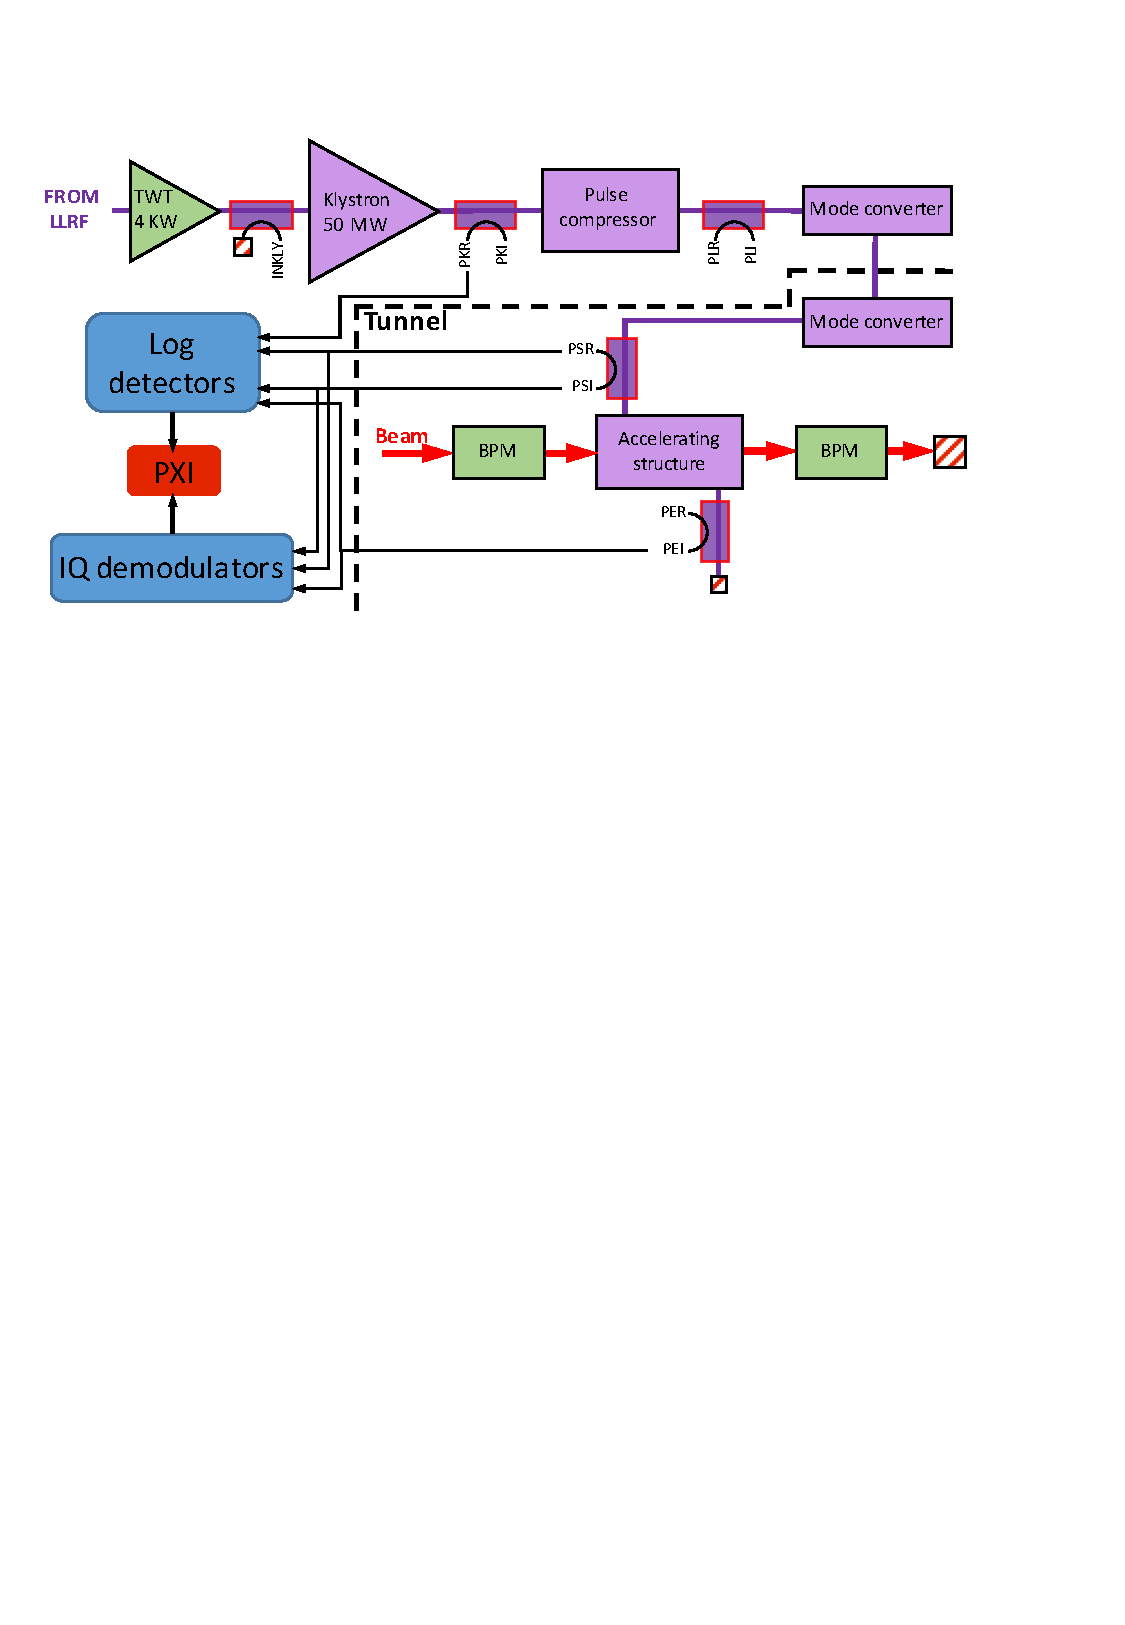
\includegraphics[scale=0.8]{pictures/high-level-RF-scheme.pdf}
\caption{Schematic of the high level RF and the relevant part of the DAQ for the interlock system. See appendix for glossary of abbreviations}
\label{high_l_RF}
\end{figure}



\subsection[Online triggers]{Online triggers}
 \label{subs:itlk}

An interlocking system is implemented in the PXI crate, in order to detect the breakdown events and trigger the data saving. When one of the interlocks is triggered, it acts on the LLRF power, cutting the power but leaving the rest of the amplification chain ready. After a period of time, generally seconds, the power is restarted and ramped up gradually.

There are four interlocks of this kind, triggered when one of the following quantities exceedes a user-defined threshold:
\begin{enumerate}
\item {\makebox[7cm]{Cavity peak reflected power:\hfill} $max(P_{REF})$}
\item {\makebox[7cm]{Cavity reflected energy:\hfill} $\int P_{REF}(t) \, dt $}
\item {\makebox[7cm]{Cavity missing transmitted energy:\hfill} $\int P_{INC}(t)\,dt - \int P_{TRA}(t)\,dt$}
\item {\makebox[7cm]{Peak power reflected to the klystron:\hfill} $max(P_{KREF})$}
\end{enumerate}
The last interlock is meant to protect the klystron, and is triggered when the reflected power back from the pulse compressor is too high. This happens especially when the pulse compressor is not properly tuned, as described later in this chapter.
The first three indeed are used to detect a breakdown event inside the structure under test. When one or more of these four interlock is triggered, the event is saved by the PXI crate. In addition, an event is saved every minute, to monitor the state of the current test.

Generally a breakdown event triggers more than one of the criteria above. A key point is the redundancy: any of the interlocks triggers the event recording in order to not to lose any interesting event. Additional events that trigger the saving are stored anyway, and will be filtered out during the offline analysis described in the next chapter.


\section[Other systems]{Other systems}

\subsubsection{Cooling system}

The operation of CLIC requires a component alignment on the $\mu$m scale. Once realised during the installation, the alignment has to be maintained keeping the thermal dilation under control. A number of studies have been carried out to this purpose, such as \cite{Daskalaki:2141828}. The thermal data from the accelerating structure installed in the dogleg are currently analysed as part of these studies.

The heating of the accelerating structures is provoked by the Joule heating induced by the RF encountering the resistive walls. In nominal conditions the heating is constant once the structure is running at constant RF input power. 

In this perspective the breakdown events have a key role since they modify the heating, because of the perturbation of the RF power flow. This materialises both because of the power reflection by the plasma in the accelerating cavity, and the huge amount of power absorbed by the plasma, that can achieve the level of tens of MW.


\subsubsection{Vacuum system}

In every accelerator an adequate vacuum has to be reached to preserve the quality of the beam. Compared to the traditional vacuum systems, in accelerators there are additional phenomena taking place. In fact, in addition to permeation, the desorbtion of surfaces is enhanced by beam losses and the photon emission from the beam. 

An adequate pumping system is hence necessary, and is described in \cite{ctf3:dr}.

On top of the vacuum system for the beam pipes, the waveguide network has to be kept under high vacuum. Also in this case there is an additional effect to the permeation, that is similar to the beam losses. The plasma that establishes during the breakdown process is formed by material evaporated from the cathode, and needs to be pumped out to restore the vacuum level as soon as possible. Furthermore, the vacuum arc emits electrons and ions that can enhance desorbtion.


\section[Operation of the setup]{Operation of the setup}

One of the main tasks of the author of the thesis was to carry out the operation and supervision of the accelerator and of the 12 GHz RF production, in addition to the data analysis. It seems therefore appropriate to spend some words on the operation and the operational issues encountered in the CTF3.

\subsection{Linac operation}

During 2016 the CTF3 schedule foresaw running the Drive Beam during the week and switching to the Main Beam for the weekend. The reason is that the high-gradient testing experiments require a long beam time to collect data, because of the low breakdown rates. So they are be carried out by leaving the accelerator running when it is not in use by other operators. A reliable system of interlocks is diagnosing the equipments and ensuring the protection of the accelerator. 

As mentioned before, the linac of the CTF3 is normally operated in fully-loaded mode, producing a long  high-current beam pulse of the Drive Beam. In order to produce the Main Beam for the BD tests, it is necessary to produce a short beam pulse with a lower current and a resulting higher energy. 

The accelerating structures in the linac are powered by 45 MW klystrons equipped with pulse compressor system. 
The RF pulse shape is changed by modifying the phase program of the low level RF.

The current pulse duration from the gun is also adapted to the new beam. The beam optics was calculated to minimise the beam size in the accelerating structure, and the quadrupole gradients are set up accordingly.

This operation required normally slightly less than an hour, mainly due to temperature settling of the RF pulse compressors, sometimes up to a couple of hours.

The operation has to be supervised during the running, since the trip of some component can cause an interruption of the beam or of the RF production. The operation has been automatised to restart after the most common trips without operator intervention. Nevertheless, other faults have to be dealt with manually. The typical uptime without intervention is around one day.

\subsection{Xbox operation}
\label{sec:xboxop}

The repetition rate used is 25 or 50 Hz, to accumulate higher statistics.

After a breakdown, the power is stopped as foreseen in the CLIC operational scenario. After the stop, the power is gradually ramped up. Overall, the power restoration lasts less than 10 s if no other breakdown happen.

Power dissipation changes leads to detuning of the pulse compressor. The detuning can be provoked by frequent breakdowns (which stops the RF production),  switching from loaded to unloaded condition (normally because of problems on the linac; the RF input power level is lowered in some cases when there is no beam), or from the thermal day-night excursion. The pulse compressor detuning is accompanied by the increase of reflections to the klystron. A tuning algorithm has been implemented to face this effect. More details about the tuning will be given in section \ref{sec:PCtune}.
\clearemptydoublepage
\chapter[Data analysis]{Data analysis}

\section[Offline selection of the events]{Offline selection of the events}

In order to perform the data analysis, a full analysis framework have been developed using MATLAB. The selection of the interesting events will be described chronologically, as it's performed in the analysis program.

\subsection[Data collected from the PXI]{Data collected from the PXI}

As mentioned in the previous chapter, the data acquisition is performed from a real-time LabVIEW program running into the PXI crate. When an event hits at least one of the online triggers is saved into the crate's disk. Every 8 hours, the crate assemble a data file and stores it in TDMS format \cite{NI:TDMS}. To proceed with the analysis, the files are merged joining all the data of the same day together in a new data file. The original data are anyway kept stored. All these actions were found already implemented in the system at the beginning of this work.

The kind of events that are collected by the PXI crate have two natures:
\begin{enumerate}
\item Interlock pulses: an event that triggered one of the online interlock. If available, the two precedent pulses are saved.
\item Backup pulses: if no event triggers an online interlock, a pulse every minute is saved.
\end{enumerate}
The first ones are sent to the next analysis step, the second ones are analysed separately to check the running condition of the accelerator and the RF systems.


\subsection[Power spikes detection]{Power spikes detection}

A key operational issue is the presence of power spikes, that sometimes are detected in the systems. The main characteristics of these events are:
\begin{itemize}
\item Short duration: normally in the range 10-100 ns
\item Very high power burst: it can reach 60-70 MW or even more 
\end{itemize}
The fist point makes the spikes easily detectable using a frequency filter to detect signals of that short duration. 

 After careful investigation, the origin of the spikes has been addressed to the TWT. It has to be pointed out that the frequency of the spikes is anyway low compared to the rate of the breakdown, and that after the first runs the replacement of a very active tube improved a lot the performance. As can be seen in Fig. \ref{spikesAndDetuning}, the spike can happen everywhere in the pulse.

 \begin{figure}[h]
 \centering
   \subfigure[Power spike in the prepulse]
   {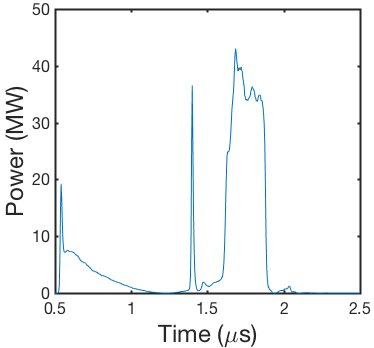
\includegraphics[scale=0.48]{pictures/spike1.png}}
 \hspace{2mm}
 \subfigure[Power spike in the compressed pulse]
   {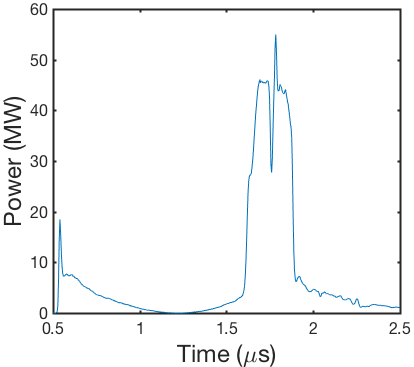
\includegraphics[scale=0.46]{pictures/spike2.png}}
 \caption{Cavity input power signal for two different spikes. Spikes can happen anywhere in the signal, even if the experience suggest that are more likely in the compressed pulse.}
 \label{spikesAndDetuning}
 \end{figure}


When a spike gets detected, the correspondent interlock is sorted out, and also the followings for a given period of time (generally 90 s). The reason is that it is believed that the burst of power brought from the spike may trigger strong breakdowns that damage the surface. This creates new emitters that triggers new breakdowns as soon as the system don't reach an equilibrium. The waiting time before restarting to count the breakdowns gives time to the surface to cool down and get reconditioned.


\subsection[Pulse compressor tuning issues]{Pulse compressor tuning issues}

RF tests of accelerating cavities are carried out using the CLIC nominal pulse shown in Fig. \ref{detuning_fig} (a). This comes from the necessity to find a common test protocol for accelerating cavities, that has also to match the different pulse length of the RF foreseen in the three stages of the CLIC implementation. To meet these requirements, the CLIC nominal pulse is made of a filling (or rising) time of 70 ns and a flat-top 180 ns long.

A common operational issue is the detuning of the pulse compressor, that provokes an imperfect shape of the RF pulse. This event does not constitute an issue for the implementation of CLIC (unless implemented in the klystron option). Anyway excessively detuned running periods are sorted out, hence far from the wanted experimental conditions. 

The origin of the detuning is the difference of the total volume of the pulse compressor's cavities. This is controlled changing the cooling water temperature, but as any other thermal system needs time for the regulation \cite{Woolley:CWS2016}. The detuning is a particular issue in summer, when the thermal excursion during the day is particularly high.

As general rule a slight detuning of the pulse is tolerated, and it is not possible to get rid of it because the regulation of the temperature of the chillers act dynamically and needs time to compensate the variations. On the other hand the data are not considered in case of extreme detuning such as in Fig. \ref{detuning_fig} (b) and (c), where the box-shape of the pulse is not recognisable anymore. 

 \begin{figure}
 \centering
  \subfigure[CLIC nominal pulse]
   {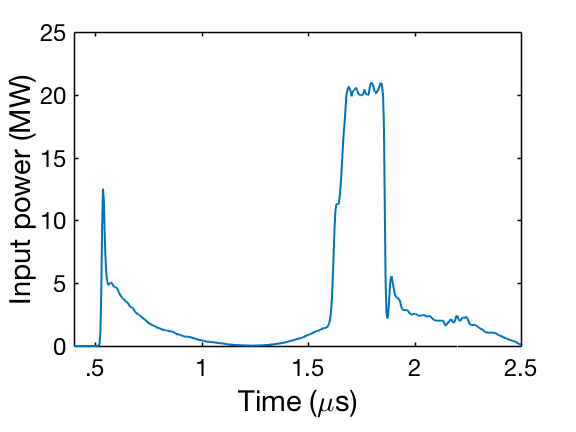
\includegraphics[scale=0.45]{pictures/CLIC_nominal_pulse.png}}
  \subfigure[Pulse compressor undertuned]
   {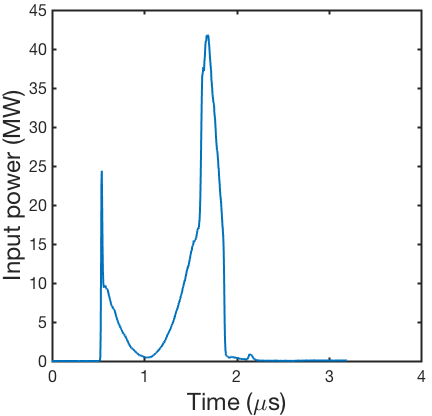
\includegraphics[scale=0.42]{pictures/Undertuning.png}}
 \hspace{2mm}
 \subfigure[Pulse compressor overtuned]
   {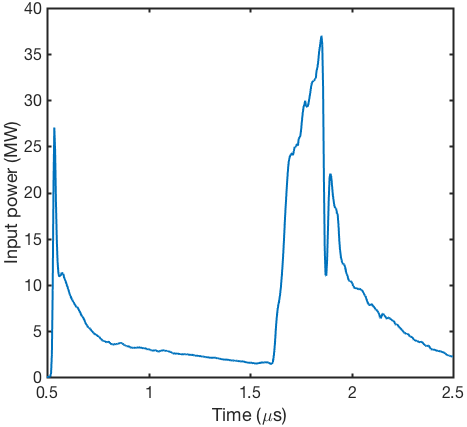
\includegraphics[scale=0.41]{pictures/Overtuning.png}}
\caption{The CLIC nominal pulse and two extreme cases of detuning of the pulse compressor.}
 \label{detuning_fig}
 \end{figure}


\subsection[The metric]{The metric}

The key issue in the analysis of the vacuum arcs in the accelerating cavity is to understand if the breakdown happened in the accelerating cavity, and sort out the breakdowns happening elsewhere. For this purpose two quantities are evaluated:
\begin{equation}
\frac{ E_{INC} -  E_{REF}   }{  E_{INC} +  E_{REF}   }
\end{equation}
\begin{equation}
\frac{ E_{INC} -  E_{TRA}   }{  E_{INC} +  E_{TRA}   }
\end{equation}
by doing so two distinct regions gets highlighted (see Fig. \ref{Metric_plot}). The upper left region is made of the fake interlocks and the breakdown that happen upstream the structure under test. The events happening in the structure end up in the lower right area on the plot.

\begin{figure}[h]
\centering 
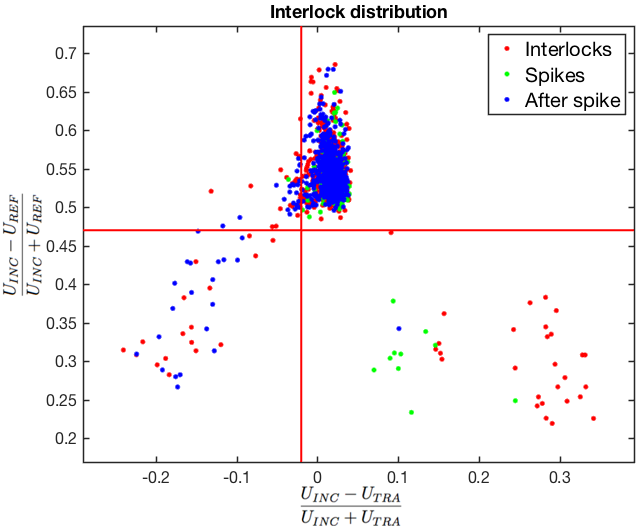
\includegraphics[scale=0.6]{pictures/metric_plt.png}
\caption{Metric plot for an unloaded run. Data grouped in two different regions are clearly visible. The lowest region is containing the interesting interlocks, that are sent to the next analysis step}
\label{Metric_plot}
\end{figure}


The selection based on the metric would be already sufficient to produce good results, with no need of further refining.



\subsection[Additional criteria for runs with beam]{Additional criteria for runs with beam}

During the experiments with beam, two additional conditions have to be met to consider an interlock as a breakdown in the accelerating structure
\begin{enumerate}
\item The beam has to be present during the pulse
\item In the case of a breakdown happened during a period without beam, the 
\end{enumerate}











\section[Time and space positioning of the breakdowns]{Time and space positioning of the breakdowns}







\section[Beam induced RF]{Beam induced RF}

\clearemptydoublepage
\chapter[Results and future developments]{Results and future developments}

\section[Measurements summary]{Measurements summary}

\subsection[Input power levels]{Input power levels}

A number of measurements have been collected during 2016. Figure \ref{g_IP} shows the relation between the average gradient and the input power in the accelerating structure. The measurement points have been selected to allow the comparison between the different running conditions, as outlined in Chap. \ref{chap:motivation}, and are summarised in Table \ref{run_pwr}.

\begin{table}
  \centering
    \begin{tabular}{ c l }
    \hline
    \hline
    Run type		&	Input power (MW)		\\
    \hline
    unloaded 		&	43.3, 41, 38 and 24.6	\\
    loaded			&	43.3, 41 and 38			\\
    anti-loaded		&	6.5					\\
    \hline
    \hline
    \end{tabular}
\caption{Input power levels of measurements in 2016.}
\label{run_pwr}
\end{table}

The measurements at different input power level have not been taken in a precise order, anyway it has been tried to keep long measurement periods as much as possible at the same input power. 
The choice is normally complicated by the fact that the Xbox was not able to provide the maximum RF power level during the year, mainly because of technical problems. The order of the runs at constant input power is reported in Fig. \ref{BDR ALL, in appendix ???}.


\subsubsection{Comparison of loaded and unloaded runs at same average gradient}

For the CLIC test purpose,  carry out a measurement at 100 MV/m average gradient comparing loaded and unloaded runs would be the most interesting measurement possible. In order to perform it, the input power has to raised from 43.3 MW in the unloaded case to 67.5 MW in the loaded case. 

Unfortunately it was clear from the beginning that reaching 67.5 MW of input power was not possible because the waveguides that deliver the power from the pulse compressor to the structure under test are not conditioned for such high power flux.

Because of this limitation, the choice comes down to perform measurements at the same input power and compare the results. 

During a period of technical problems, it has been anyway collected an unloaded measurement at 24.6 MW of input power, in order to compare it with the correspondent average gradient in the loaded case at 43.3 MW of input power. Unfortunately with a such low input power, the breakdown rate is very low, and after 4 days of measurements zero breakdowns were collected. Therefore it is only possible to affirm that running unloaded at 24.6 MW input power, the breakdown rate is $< 7.7 \, 10^{-8} $ BD pulse$^{-1}$. 


\subsubsection{Comparison of loaded and unloaded conditions at same input power}

Most of the measurements carried out during 2016 campaign were comparing the loaded and unloaded running condition. The input power levels used were 43.3, 41 and 38 MW. It was not possible to go at lower input powers because the breakdown rates becomes so low that the data collection takes weeks to produce a sufficient statistics.


\subsubsection{Study of the antiloaded runs}

The antiloaded measurements were carried out at 6.5 MW of input power. The reason is that with a beam current  of 1.6 A, the output gradient of the structure is already around 100 MV/m (see Fig. \ref{3grad}). The results were indeed interesting and will be shown later when it comes to talk about the breakdown distribution.




\begin{figure}[t]
\centering 
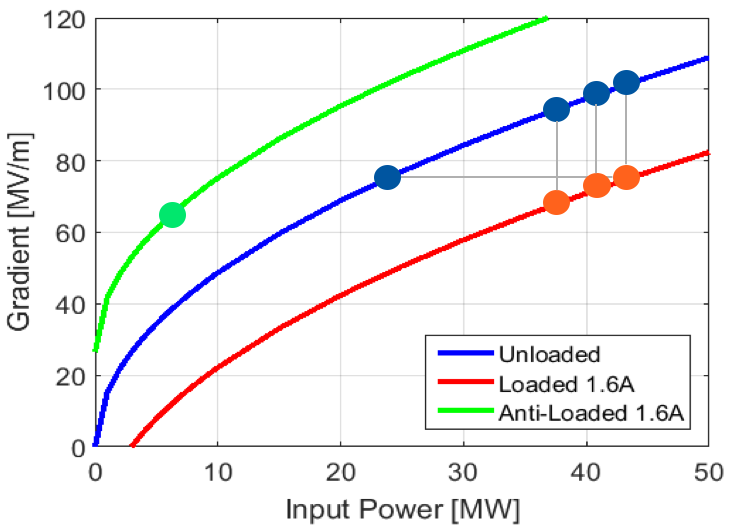
\includegraphics[scale=0.7]{pictures/grad_vs_inPow.png}
\caption{Average gradient as function of the input power in different running conditions. See text for details on the measurement points. }
\label{g_IP}
\end{figure}


\subsection[Beam pulse parameters]{Beam pulse parameters}

As mentioned in the motivation of the experiment, the goal is to understand the effect of the beam on the breakdown rate. The beam parameters have been therefore selected in order to enhance the effect of the beam, rather than try to simulate the CLIC operation. This materialises in:
\begin{itemize}
\item Higher beam current than CLIC: 1.6 A instead of 1.2 A.
\item Longer beam pulse: the beam is lasting during all the compressed RF pulse, for 250 ns, instead of last just during the flat-top of the CLIC pulse (see Sec. \ref{sec:PCtune}).
\end{itemize}

\noindent
The loaded operation is clearly visible  in the RF signals, as shown in Fig.~\ref{RF_load}.

\begin{figure}[h]
\centering
  \subfigure[Loaded operation]
   {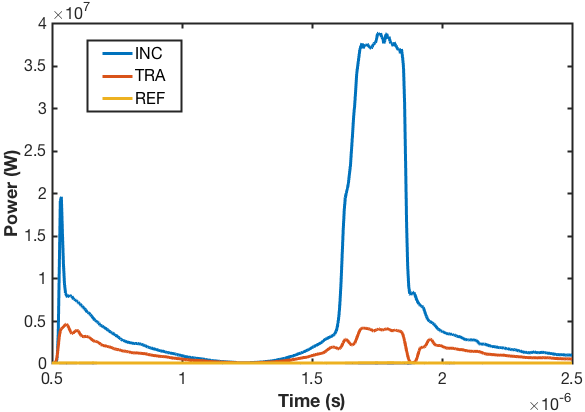
\includegraphics[scale=0.33]{pictures/LoadedPulse.png}}
  \subfigure[Antiloaded operation]
   {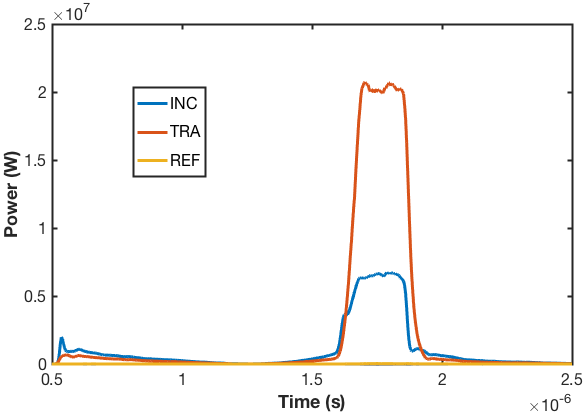
\includegraphics[scale=0.33]{pictures/AntiloadedPulse.png}}
\caption{Comparison of the RF signals during the loaded and antiloaded operation. During the loaded operation it can be observed that the transmitted power falls close to zero, because of the energy subtracted from the beam. The opposite behaviour can be noted in the antiloaded case, where the input power is much lower than the transmitted. In this case the difference in energy is provided by the beam, that gets slowed down because of the wrong phase with the RF. }
 \label{RF_load}
 \end{figure}




\section[Results]{Results}

\subsection[Breakdown distribution]{Breakdown distribution}



\subsection[Beam induced RF]{Beam induced RF}

Measurements at different input power level have been carried out during 2016. 




\section[Further developments]{Further developments}


RF:
- TWT already eliminated (no spikes anymore)
- I suggest to switch the pulse compressor to a SLED-II type, which is more stable, avoiding all the tuning problems we had
- ?


\section{Conclusions}

During the measurement campaign of this year we learnt how to operate and measure the breakdown rate of the structure with and without beam.

The beam effect analysis has still to be carried on in detail, in particular have to be understood if when running with beam the conditioning takes place or not. Further investigations on this topic require a stable and extensive beam time, which was not the case of the CTF. The comparison of this data with the ones of a stable long test with beam can suggest that switching condition ripetutamente w/ w/o beam can lead to a higher BDR ...
- as DC tests suggest
- as we cannot see because of the low rep.rate



shown effect on the migration !
\clearemptydoublepage


%%%% TAIL OF THE DOCUMENT
\backmatter
%\input{tail/aknowledgments}
%list of abbreviations
\clearemptydoublepage
\chapter*{List of Abbreviations}

\begin{tabular}{l l}
BPM		&	Beam Position Monitor\\
CDR		&	Conceptual Design Report\\
CERN	&	Conseil europ\'een pour la Recherche nucl\'eaire, Geneva, Switzerland\\
CLIC		&	Compact Linear Collider\\
CTF3	&	CLIC test facility 3\\
EEE		&	Explosive Electron Emission\\
EFE		&	Enhanced Field Emission\\
EM		&	Electromagnetism \textit{-or-} electromagnetic\\
FCC-ee	&	Future Circular Collider, lepton version\\
FCC-hh	&	Future Circular Collider, hadron version\\
FE		&	Field Emission\\
FOM		&	Figure Of Merit\\
HOM		&	High(er) Order Mode\\
ICFA		&	International Committee for Future Accelerators\\
ILC		&	International Linear Collider\\
KEK		&	High Energy Accelerator Research Organization, Tsukuba, Japan      \\  
LEP		&	Large Electron Positron Collider\\
LHC		&	Large Hadron Collider \\
LINAC	&	Linear Accelerator\\
LLRF	&	Low-level RF\\
NC		&	Normal Conducting\\
PETS	&	Power Extraction and Transfer Structure\\
RF		&	Radio frequency\\
SC		&	Super Conducting\\
SLAC	&	Stanford Linear Accelerator, Menlo Park, California\\
SM		&	Standard Model\\
SPS		&	Super Proton Synchrotron\\
SWS		&	Standing Wave Structure\\
TBM		&	Two-Beams module\\
TDR		&	Technical Design Report\\
TE		&	Transverse Electric (modes of a WG)\\
TM		&	Transverse Magnetic (modes of a WG)\\
TWS		&	Travelling Wave Structure\\
TWT		&	Travelling Wave Tube\\
WG		&	Waveguide\\
XBOX	&	X-band high power RF test stand\\
\end{tabular}
\clearemptydoublepage
%list of figures
\listoffigures
\clearemptydoublepage
%list of tables
\listoftables
\clearemptydoublepage
%bibliography
\addcontentsline{toc}{chapter}{Bibliography}
\bibliography{bibliography/bibThesis}
\bibliographystyle{ieeetr}
\clearemptydoublepage


\end{document}
